
\pagestyle{plain}

\section{Estado de la cuestión}
La contabilidad, con el paso del los años, se ha vuelto cada vez más complicada. Con la explotación de las tecnologías en auge a lo largo de este siglo XXI, no solo ha provocado que haya más datos distribuyéndose por la red, sino que también cada vez sea más fácil realizar transacciones. La facilidad de hoy en día en cuanto a viajar y comunicarse con otros clientes, permite a las empresas cada vez ir expandiéndose más. Las compras \ti{online}, junto con que cada vez hay soluciones más específicas para cada tarea, también le añaden una capa de complejidad mayor a la contabilidad. Esto genera una necesidad vital de tener que depender de una o de varias herramientas informáticas para poder llevar a cabo esta tarea tan fundamental en una empresa.

No solo estas herramientas software facilitan el trabajo a las personas en este departamento haciendo los procesos contables más rápidos y precisos, sino que también abren puerta al análisis y exploración de los datos contables. Con esto, se puede adquirir un conocimiento mucho más profundo de la situación de la empresa y de cómo afrontar y determinar el futuro de esta. 

En esta sección se explicarán, en una primera instancia, conceptos de contabilidad necesarios para entender el desarrollo de este trabajo. Una vez finalizado este apartado, se tratará un apartado BI/BA donde se profundizará más en características de los datos como su tipo, almacenamiento y visualización. Además, la parte teórica se cerrará explicando la sección de inteligencia artificial. Por último, se comentarán algunos trabajos relacionados con este mismo.

\subsection{Marco teórico del trabajo}
\subsubsection{Contabilidad}
Para poder llevar a cabo toda la información financiera de la empresa, la contabilidad recoge las transacciones diarias en lo que se denomina \B{Libro Diario}. Cualquier transacción afecta mínimo a dos cuentas. Por ejemplo, la compra de un producto por parte de la empresa, afecta a la adquisición de este producto por un parte (cuenta 1) y al proveedor a quien se le compra este producto (cuenta 2). Hay distintos tipos de cuentas y todas ellas tienen un número asociado. Este número asociado a cada cuenta es el mismo en todas las empresas españolas para todas las  cuentas. Esto es porque dichas cuentas están regularizadas por el \B{Plan General Contable} (PGC) de España.

Para explicar de la mejor manera posible conceptos posteriores, se divide estas cuentas de la siguiente manera:
\
\subsubsubsection{Cuentas Activo, Pasivo y Patrimonio Neto}

\B{Activo}

El \B{activo} se refiere al conjunto de bienes y derechos que una empresa posee en un determinado momento.
Se puede dividir en:
\begin{itemize}
	\item \B{Corriente} (corto plazo): dinero en caja, dinero en banco, inventario, etc.
    \item \B{No corriente} (largo plazo): terrenos, edificios, vehículos, etc.
\end{itemize}
Por lo general, largo plazo (l/p) se suele considerar un periodo de tiempo de más de un año y corto plazo (c/p) un periodo de tiempo menor a un año.

\bigskip

\B{Pasivo} 

El \B{pasivo} se refiere al conjunto de deudas y obligaciones a pagar por la empresa. Al igual que el activo, el pasivo puede ser:
\begin{itemize}
	\item \B{Corriente} (corto plazo): deuda a un proveedor a pagar en menos de un año o retenciones de IRPF practicadas a empleados o proveedores, etc.
    \item \B{No corriente} (largo plazo): e.g. deuda con el banco de un préstamo a cuatro años.
\end{itemize}

Un aspecto importante que el departamento de contabilidad deberá tener en cuenta, es que el pasivo corriente no deberá ser mayor al activo corriente, pues sería un indicativo de que la empresa tendrá un problema financiero a corto plazo.

\bigskip

\B{Patrimonio Neto}

El \B{patrimonio neto} es un indicativo de la salud de la empresa. En otras palabras, el patrimonio neto es básicamente el $activo  - pasivo$. Por tanto, una empresa debería buscar siempre tener un patrimonio neto positivo; y cuanto mayor sea este, mejor.

\bigskip

\B{Balance general}

El \B{balance general} ---también llamado balance de situación--- es un documento que refleja la situación de la empresa en términos monetarios en un momento determinado. El balance es pues, como una fotografía o resumen instantáneo de la situación de la empresa \parencite{libroContabilidad}. En este documento, están reflejadas las tres cuentas que recién se han mencionado en este apartado. Está dividido en dos columnas: activos en la columna de la izquierda; y, por otro lado, pasivo y patrimonio neto en la columna de la derecha (véase la Figura \ref{balance}).


\begin{figure}[H]
    \centering
    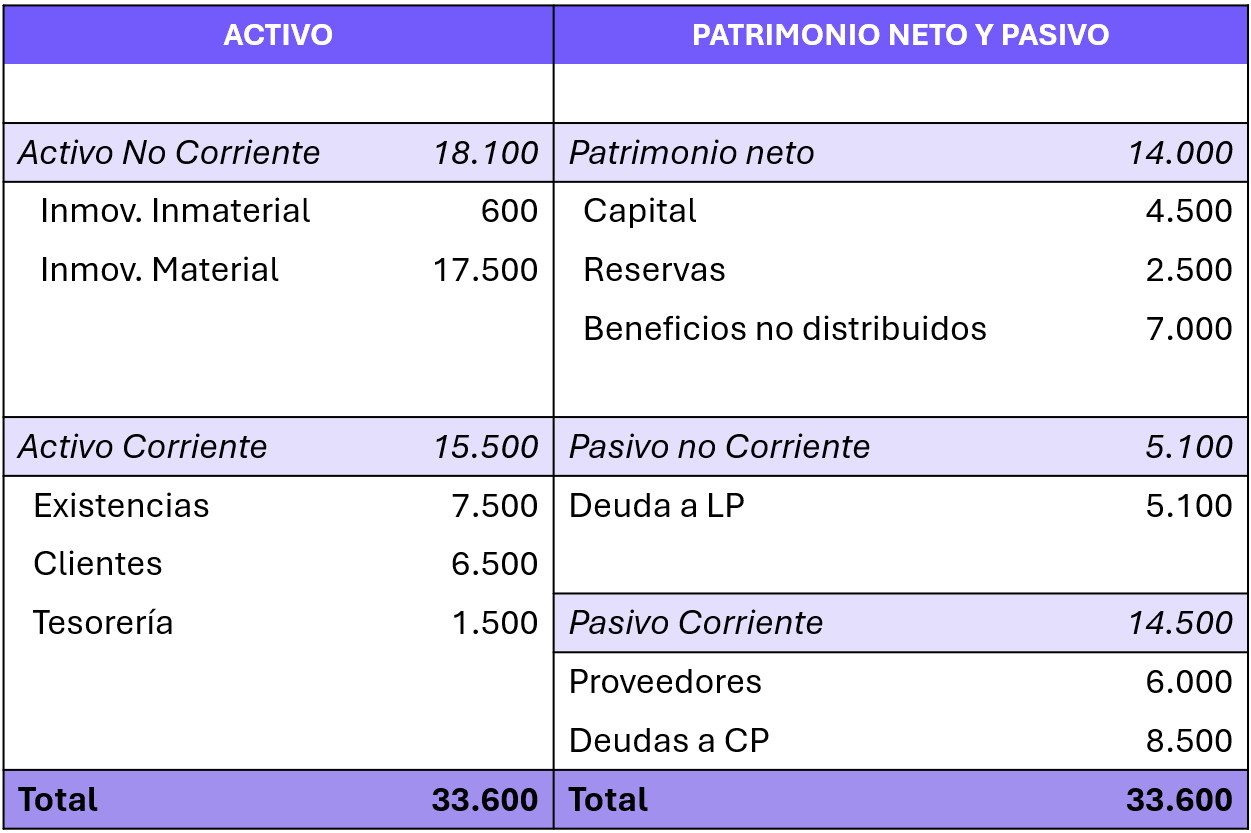
\includegraphics[scale = 0.5]{imgs/balance.png}
    \caption{Ejemplo balance general. \ti{LP = largo plazo, \hspace{0,1cm} CP = corto plazo}.}
    \label{balance}
\end{figure}


Algo a tener en cuenta es, que la suma de los elementos de la columna izquierda (activo) es igual a la suma de los elementos de la derecha (pasivo y patrimonio neto). Esto se conoce como \B{la ecuación fundamental de la contabilidad}:
\begin{equation*}
    \text{Activo} = \text{Pasivo} + \text{Patrimonio neto}
\end{equation*}

La columna de la derecha se dice que es el \B{origen de fondo} de una empresa. Es decir, de ahí provienen los recursos para adquirir los activos de una empresa. Luego, la columna de la izquierda se dice que es la \B{aplicación} de dicho fondo. 

\subsubsubsection{Cuentas de compras / gastos y ventas / ingresos}
El balance de situación, como se ha mencionado, sirve para proveer información acerca de la situación de la empresa en un momento dado. Pero este documento es informativo, no orientativo. En cambio, para saber si la empresa está generando  beneficios en un periodo de tiempo concreto, es la \B{cuenta de resultados} la que informa acerca de esto. 

\bigskip

\B{Compras y gastos}

La cuenta de compras y gastos es la que la empresa emplea para registrar la compra de existencias ---i.e. productos que la empresa compra para luego  venderlos\fnm---; así como los gastos que esta tiene como consecuencia de su actividad. Estos gastos son muy variados, pero los más comunes son: los sueldos que se pagan a los empleados, facturas de la luz, alquiler, etc.
\fnt{Cabe remarcar que esto es así porque se va a emplear el procedimiento especulativo de cuenta divisionaria\textsuperscript{\hyperref[ap:pecd]{A1}}. Se recomienda leer el siguiente punto \ref{PGC} antes de ir al apéndice.}

\bigskip

\B{Ventas e Ingresos}

La cuenta de ventas e ingresos es justo la opuesta. Esta cuenta se emplea cuando la empresa vende alguna mercadería previamente adquirida a algún proveedor; así como los ingresos que la empresa genere más allá de estas ventas, como puede ser el alquiler de una planta de su edificio a otra empresa, prestación de servicios, etc.

\bigskip

\B{Cuenta de resultados}

Es a través de estas dos cuentas, con las que es posible realizar la cuenta de resultados. Este documento, a diferencia del balance general, no es informativo, sino que es orientativo. Es decir, a través de este documento se sabe si la empresa está generando ganancias, o, por el contrario, pérdidas. La ecuación para calcular la cuenta de resultados es bastante trivial\fnm:
\begin{equation*}
    \text{Cuenta de Resultados} = \text{Ingresos} - \text{Gastos}
\end{equation*}
\fnt{Debido al procedimiento especulativo de cuenta divisionaria, habría que añadir la variación de existencias (cuenta 610) a la ecuación, pero no se va a entrar en tanto detalle en este trabajo.}

\subsubsubsection{Plan General Contable}
El Plan General Contable (PGC) es un estándar que siguen las empresas en su contabilidad. Se puede definir como el diccionario de la contabilidad, pues se encarga de asignar un \B{número concreto} a cada cuenta. Es decir, por ejemplo, la cuenta de compras y gastos tiene el número asociado 6XX. Dependiendo del tipo de compra o gasto, la operación tendrá un número más concreto. Dos ejemplos muy comunes son la cuenta 600 asignada a la compra de mercaderías y la cuenta 640 para los salarios que se pagan a los empleados ---son un gasto para la empresa---. En definitiva, la cuenta de compras y gastos es una sección (grupo) del PGC\fnm; y esta sección está dividida en subsecciones para diferenciar unos gastos de otros. Pero la cuenta de compras y gastos no es la única.
\label{PGC}
\fnt{Se deja en el \ti{apéndice}\textsuperscript{\hyperref[ap:pgc]{A2}} el PGC algo más detallado sobre qué es cada grupo, así como los números de cuentas ---i.e. subgrupos--- más empleados.}
\begin{figure}[H]
    \centering
    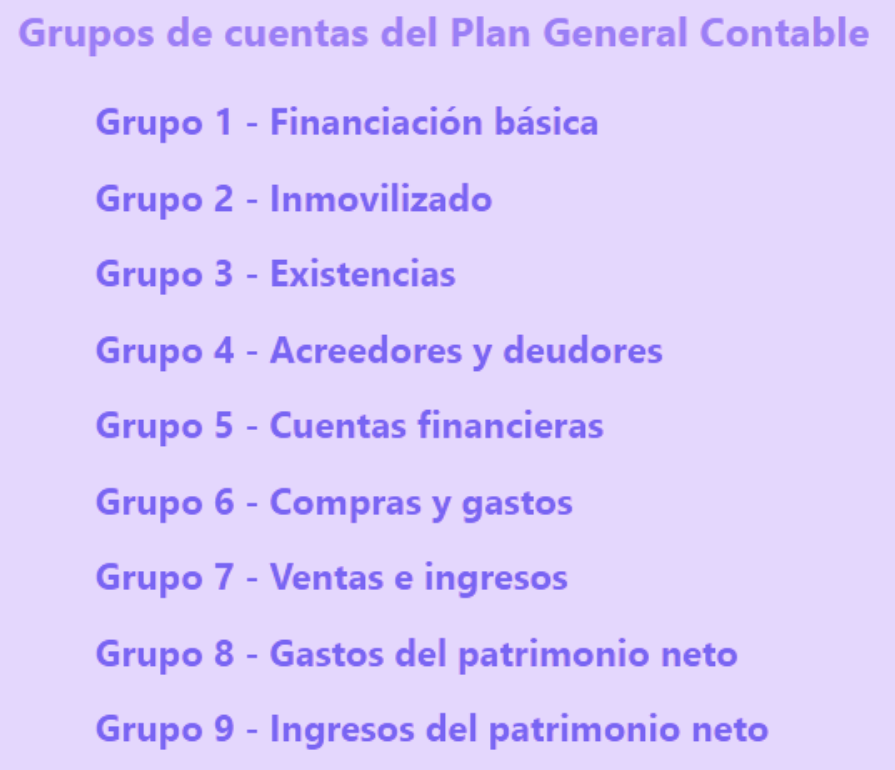
\includegraphics[scale = 0.4]{pgc}
    \caption{Secciones del Plan General Contable español. \scriptsize{Fuente: \url{https://www.plangeneralcontable.com}}}
    \label{pgc}
\end{figure}

De la Figura \ref{pgc}, el grupo 6 y grupo 7 son las cuentas de compras/gastos y ventas/ingresos que se han mencionado en el apartado anterior. Por tanto, en el grupo 6 irán a parar todas aquellas transacciones relacionadas con las compras y gastos, como puede ser la factura de la luz; mientras en el grupo 7 quedarán registradas las transacciones de ventas/ingresos, como  puede ser la prestación de servicio a una empresa. Las otras tres cuentas restantes del apartado anterior ---i.e. activo, pasivo y patrimonio neto--- están algo repartidas porque cubren muchas transacciones distintas. Las de patrimonio neto se encuentran principalmente en el grupo 1, grupo 8 y grupo 9. Los activos, en cambio, están distribuidos sobre todo en el grupo 2, grupo 3, grupo 4 y grupo 5. Los pasivos están mayoritariamente en los grupos 1 y 5.

\subsubsubsection{Libro Mayor}
Cada una de estas cuentas, siempre que se haga una operación que la involucre, quedará registrada en el \B{Libro Mayor}. Este, por lo general, suele "empezar de cero" a inicio de año. Cada cuenta tiene la siguiente estructura:
\begin{figure}[H]
    \centering
    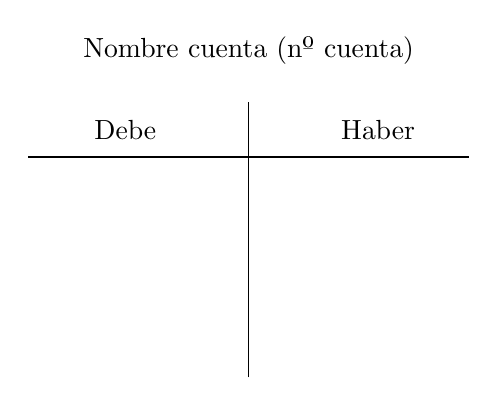
\begin{tikzpicture}[scale=0.7] 
        % Línea vertical
        \draw (0,0) -- (0,5);
        % Línea horizontal
        \draw (-4,4) -- (4,4);
        \node[left] at (-1.5,4.5) {Debe};
        \node[right] at (1.5,4.5) {Haber};
        \node[above] at (0,5.5) {\B{Nombre cuenta (nº cuenta)}};
    \end{tikzpicture}
    \caption{Estructura de una cuenta en el Libro Mayor.}
    \label{LM}
\end{figure}
La Figura \ref{LM} es la representación de una cuenta en el Libro Mayor. Dicha cuenta se indica arriba con el nombre de la cuenta y su número. Si se hace una anotación en el debe, se dice que se \B{carga la cuenta}. De lo contrario, si se hace una anotación en el haber, se dice que \B{se abona}. Estas cuentas, como ya se ha visto, pueden ser de 4 tipos: activo, pasivo (pasivo y patrimonio neto), compra/gasto y venta/ingreso. De manera breve, las cuentas de activo funcionan igual que las cuentas de compra/gasto; y dichas cuentas son opuestas a las de pasivo y ventas/ingresos respectivamente. 

\bigskip

\B{Debe y Haber en el activo y pasivo}

Cuando la cuenta de un activo aumenta, este aumento queda reflejado en el \B{Debe}. En cambio, cuando disminuye, esto se anota en el \B{Haber}. De manera antagónica funcionan las cuentas de pasivo. Véase la Figura \ref{LMAP}.


\begin{figure}[H]
    \centering
    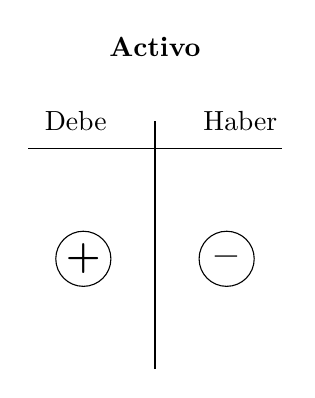
\begin{tikzpicture}[scale=0.7] 
        % Primera tabla
        % Línea vertical
        \draw (0,0) -- (0,4.5); % Cambio de coordenadas finales
        % Línea horizontal
        \draw (-2.3,4) -- (2.3,4); % Cambio de coordenadas finales
        \node[left] at (-0.7,4.5) {Debe};
        \node[right] at (0.7,4.5) {Haber};
        \node[above] at (0,5.5) {\textbf{Activo}};
        \draw (-1.3,2) circle (0.5cm);
        \node at (-1.3,2) {\textbf{\Large +}};
        \draw (1.3,2) circle (0.5cm);
        \node at (1.3,2) {\textbf{\Large --}};
    \end{tikzpicture}
    \hspace{2cm} % Espacio entre las dos tablas
    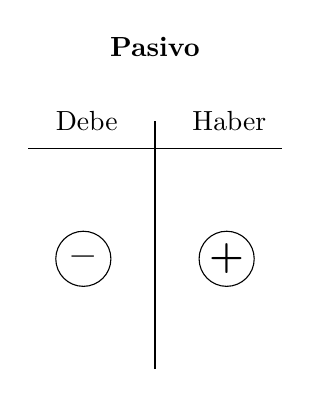
\begin{tikzpicture}[scale=0.7] 
        % Segunda tabla (igual a la primera)
        % Línea vertical
        \draw (0,0) -- (0,4.5); % Cambio de coordenadas finales
        % Línea horizontal
        \draw (-2.3,4) -- (2.3,4); % Cambio de coordenadas finales
        \node[left] at (-0.5,4.5) {Debe};
        \node[right] at (0.5,4.5) {Haber};
        \node[above] at (0,5.5) {\textbf{Pasivo}};
        \draw (-1.3,2) circle (0.5cm);
        \node at (-1.3,2) {\textbf{\Large --}};
        \draw (1.3,2) circle (0.5cm);
        \node at (1.3,2) {\textbf{\Large +}};
    \end{tikzpicture}
    \caption{Ejemplo cuentas activo y pasivo Libro Mayor.}
    \label{LMAP}
\end{figure}

La Figura \ref{LMAP} se puede interpretar como que las columnas de la izquierda (Debe) cuanto más aumenten, mejor para  la empresa ---pues supone más activo y menos deuda respectivamente---. Justo lo contrario ocurre con las columnas de la derecha (Haber). A final de año, cuando se evalúen estas cuentas, si el Debe en una cuenta es mayor al Haber, se dice que la cuenta presenta un saldo \B{deudor}. De lo contrario, la cuenta presenta un saldo \B{acreedor}. En caso de que el Debe y el Haber sean iguales, entonces la cuenta presenta \B{saldo cero}.

\bigskip

\B{Debe y Haber en la compra/gasto y venta/ingreso}

Estas cuentas son análogas a las anteriores. Es decir, quedarían de la siguiente manera:
\begin{figure}[H]
    \centering
    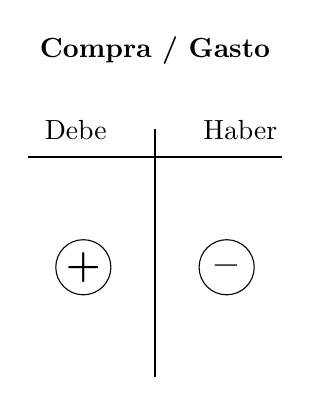
\begin{tikzpicture}[scale=0.7] 
        % Primera tabla
        % Línea vertical
        \draw (0,0) -- (0,4.5); % Cambio de coordenadas finales
        % Línea horizontal
        \draw (-2.3,4) -- (2.3,4); % Cambio de coordenadas finales
        \node[left] at (-0.7,4.5) {Debe};
        \node[right] at (0.7,4.5) {Haber};
        \node[above] at (0,5.5) {\textbf{Compra / Gasto}};
        \draw (-1.3,2) circle (0.5cm);
        \node at (-1.3,2) {\textbf{\Large +}};
        \draw (1.3,2) circle (0.5cm);
        \node at (1.3,2) {\textbf{\Large --}};
    \end{tikzpicture}
    \hspace{2cm} % Espacio entre las dos tablas
    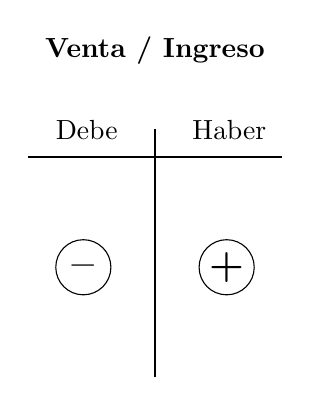
\begin{tikzpicture}[scale=0.7] 
        % Segunda tabla (igual a la primera)
        % Línea vertical
        \draw (0,0) -- (0,4.5); % Cambio de coordenadas finales
        % Línea horizontal
        \draw (-2.3,4) -- (2.3,4); % Cambio de coordenadas finales
        \node[left] at (-0.5,4.5) {Debe};
        \node[right] at (0.5,4.5) {Haber};
        \node[above] at (0,5.5) {\textbf{Venta / Ingreso}};
        \draw (-1.3,2) circle (0.5cm);
        \node at (-1.3,2) {\textbf{\Large --}};
        \draw (1.3,2) circle (0.5cm);
        \node at (1.3,2) {\textbf{\Large +}};
    \end{tikzpicture}
    \caption{Ejemplo cuentas compra/gasto y venta/ingreso Libro Mayor.}
    \label{LMCV}
\end{figure}

Tanto la Figura \ref{LMAP} como la Figura \ref{LMCV} están regidas por el \B{método de la partida doble}. Este es un principio fundamental de la contabilidad y establece que cualquier transacción económica afecta al menos a dos cuentas. Dicha transacción tiene la misma parte positiva que negativa. Por ejemplo, si se adquieren mercancías a un proveedor, la parte positiva es que la empresa adquiere dichas mercancías y la parte negativa es que hay que pagarlas. Otro ejemplo es el pago de una deuda: la parte negativa es el gasto que supone y la parte positiva es que la empresa se ha deshecho de la deuda. Como consecuencia de esto, el \B{balance general es siempre cero} (como ya se vio en la Figura \ref{balance}). 

En la siguiente sección se presenta un ejemplo sencillo de esto que se acaba de mencionar.

\subsubsubsection{Libro Diario y asientos contables}
El Libro Mayor ---que recoge todas las operaciones llevadas a cabo por la empresa durante un periodo de tiempo--- no es más que el resultado de operaciones diarias de la empresa. Estas operaciones diarias están registradas en el \B{Libro Diario}. En otras palabras: el Libro Mayor es la consecuencia de muchos Libros Diarios. 

Las operaciones de los Libros Diarios se llevan a cabo en lo que se conoce como \B{asientos contables}. Estos asientos tienen mucho que ver con la estructura de cuentas de la sección anterior. Se dividen en Debe y Haber también, y en él están reflejados las transacciones. Cada transacción, debido al método de la partida doble, involucra al menos dos cuentas. Además, estas cuentas involucradas deben estar repartidas en Debe y Haber, de tal manera que, el dinero en dicha transacción se anule entre Debe y Haber ---i.e. cada transacción tiene la misma parte positiva que negativa, como se ha dicho con anterioridad---. Véase la Figura \ref{asiento}.
\begin{figure}[H]
    \centering
    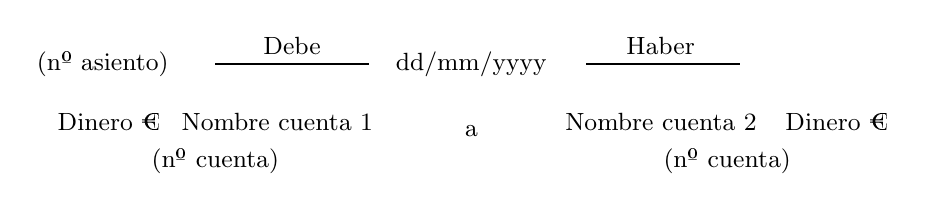
\begin{tikzpicture}[scale = 0.65]
        \node at (-6.2,0) {\B{\small{(nº asiento)}}};
        % Línea horizontal izquierda
        \draw (-4, 0) -- (-1,0);
        \node[above] at (-2.5, 0) {\small{Debe}};
        % Texto 'Operación 1' debajo de la línea izquierda
        \node[below, yshift=-0.5cm] at (-4, 0) {\small{Dinero \texteuro \hspace{0.15cm} Nombre cuenta 1}};
        \node[below, yshift=-0.5cm] at (-4, -0.7) {\B{\small{(nº cuenta)}}};
        % Centrar el texto 'a'
        \node[below,  yshift=-0.2cm] at (1, -0.7) {\B{\small{a}}};       
         % Línea horizontal derecha
        \draw (3.25,0) -- (6.25,0);
        \node[above] at (4.7, 0) {\small{Haber}};
        % Texto 'dd/mm/yyyy' en medio
        \node at (1,0) {\small{dd/mm/yyyy}};
        \node[below, yshift=-0.5cm] at (6, 0) { \small Nombre cuenta 2 \hspace{0.15cm} Dinero \texteuro};
        \node[below, yshift=-0.5cm] at (6, -0.7) {\B{\small{(nº cuenta)}}};
    \end{tikzpicture}   
    \caption{Estructura de un asiento contable.}
    \label{asiento}
\end{figure}

Para asentar los conceptos de los puntos anteriores, se va a poner un ejemplo muy simple de cómo quedaría reflejada una transacción en el Libro Diario y en el Libro Mayor. Supóngase que se compran unas mercancías a un proveedor por valor de cien euros. Esta transacción quedaría reflejada de la siguiente manera en contabilidad:

\begin{figure}[H]
    \centering
    \begin{tikzpicture}[scale=2.45]
        % Tapa izquierda
        \draw[fill=moradcl] (-3,0) rectangle (0,4);
        \node[below] at (-1.5, 4) {\B{Libro Diario}};
        % Tapa derecha
        \draw[fill=moradcl] (0,0) rectangle (3,4);
        \node[below] at (1.5, 4) {\B{Libro Mayor}};
        % Línea central
        \draw[thick] (0,0) -- (0,4);
        % Páginas en blanco
        \draw[fill=white] (-2.8,0.2) rectangle (-0.2,3.8);
        \draw[fill=white] (0.2,0.2) rectangle (2.8,3.8);
        \draw[->, bend left=30, thick] (-0.4,2.1) to (0.4,2.1);

        %######## Relleno Página izquierda #############
        \node at (-2.5, 3.65) {\tiny{Contabilidad}};
        \node at (-1.5, 0.5) {\scriptsize{\B{1}}};
        %Asiento 1
        \node at (-2.6,3.2) {\scriptsize{\B{(1)}}};
        %Debe
        \draw (-2.45, 3.2) -- (-1.65,3.2);
        \node[above] at (-2.05, 3.2) {\scriptsize{Debe}};
        \node[below, yshift=-0.5cm] at (-2.05, 3.2) {\scriptsize{100 \texteuro\hspace{0.05cm} Compra de mercancías}};
        \node[below, yshift=-1.0cm] at (-2.05, 3.2) {\scriptsize{\B{(600)}}};
        \node[below, yshift=-1.5cm] at (-2.05, 3.2) {\scriptsize{21 \texteuro\hspace{0.05cm} H.P.\fnm\ IVA soportado}};
        \node[below, yshift=-2.0cm] at (-2.05, 3.2) {\scriptsize{\B{(472)}}};
        \node[below,  yshift=-2.1cm] at (-1.5, 3.2) {\scriptsize{\B{a}}};
        %Haber
        \draw (-1.25,3.2) -- (-0.45,3.2);
        \node[above] at (-0.85, 3.2) {\scriptsize{Haber}};
        \node at (-1.45,3.2) {\scriptsize{1/1/24}};
        \node[below,  yshift=-2.1cm, align = center] at (-0.85, 3.2) {\scriptsize{  Proveedor} \hspace{0.03cm} 121 \texteuro};
        \node[below, yshift=-2.6cm] at (-0.85, 3.2) {\scriptsize{\B{(400)}}};
        %Asiento 2
        \node at (-2.6,1.5) {\scriptsize{\B{(2)}}};
        %Debe
        \draw (-2.45, 1.5) -- (-1.65,1.5);
        \node[above] at (-2.05, 1.5) {\scriptsize{Debe}};
        \node[below, yshift=-0.5cm] at (-2.05, 1.5) {\scriptsize{121 \texteuro\hspace{0.05cm} Proveedor}};
        \node[below, yshift=-1.0cm] at (-2.05, 1.5) {\scriptsize{\B{(400)}}};
        \node[below,  yshift=-1.1cm] at (-1.5, 1.5) {\scriptsize{\B{a}}};
        %Haber
        \draw (-1.25,1.5) -- (-0.45,1.5);
        \node[above] at (-0.85, 1.5) {\scriptsize{Haber}};
        \node at (-1.45,1.5) {\scriptsize{1/1/24}};
        \node[below,  yshift=-1.1cm, align = center] at (-0.85, 1.5) {\scriptsize{  Caja} \hspace{0.03cm} 121 \texteuro};
        \node[below, yshift=-1.6cm] at (-0.85, 1.5) {\scriptsize{\B{(570)}}};
       
        %######## Relleno Página derecha #############
        \node at (0.5, 3.65) {\tiny{Contabilidad}};
        \node at (1.5, 0.5) {\scriptsize{\B{2}}};
        % #####    PRIMERA FILA    #####
        % Primera tabla
        % Línea vertical
        \draw (0.45,3.0) -- (1.25,3.0); % Cambio de coordenadas finales
        \node[above] at (0.85, 3.2) {\scriptsize{\B{Compra Mercancías (600)}}};
        % Línea horizontal
        \draw (0.85,3.1) -- (0.85, 2.6); % Cambio de coordenadas finales
        \node[above] at (0.65, 3.0) {\scriptsize{Debe}};
        \node[above] at (1.05, 3.0) {\scriptsize{Haber}};
        \node at (0.40, 2.9) {\scriptsize{\B{(1) }}};
        \node at (0.65, 2.9){\scriptsize{100 \texteuro}};
        %Segunda Tabla
        \draw (1.75,3.0) -- (2.55,3.0); % Cambio de coordenadas finales
        \node[above] at (2.15, 3.2) {\scriptsize{\B{H.P. IVA soportado (472)}}};
        % Línea horizontal
        \draw (2.15,3.1) -- (2.15, 2.6); % Cambio de coordenadas finales
        \node[above] at (1.95, 3.0) {\scriptsize{Debe}};
        \node[above] at (2.35, 3.0) {\scriptsize{Haber}};
        \node at (1.7, 2.9) {\scriptsize{\B{(1) }}};
        \node at (1.95, 2.9){\scriptsize{21 \texteuro}};
        
        % #####    SEGUNDA FILA   #####
        % Primera tabla
        % Línea horizontal
        \draw (0.45,1.35) -- (1.25,1.35); % Cambio de coordenadas finales
        \node[above] at (0.85, 1.55) {\scriptsize{\B{Proveedor (400)}}};
        % Línea vertical
        \draw (0.85,1.4) -- (0.85, 0.95); % Cambio de coordenadas finales
        \node[above] at (0.65, 1.35) {\scriptsize{Debe}};
        \node[above] at (1.05, 1.35) {\scriptsize{Haber}};
        \node at (0.4, 1.25) {\scriptsize{\B{(2) }}};
        \node at (0.65, 1.25){\scriptsize{121 \texteuro}};
        \node at (1.3, 1.25) {\scriptsize{\B{ (1)}}};
        \node at (1.05, 1.25){\scriptsize{121 \texteuro}};
        %Segunda tabla
        % Línea horizontal
        \draw (1.75,1.35) -- (2.55,1.35); % Cambio de coordenadas finales
        \node[above] at (2.15, 1.55) {\scriptsize{\B{Caja (570)}}};
        % Línea vertical
        \draw (2.15,1.4) -- (2.15, 0.95); % Cambio de coordenadas finales
        \node[above] at (1.95, 1.35) {\scriptsize{Debe}};
        \node[above] at (2.35, 1.35) {\scriptsize{Haber}};
        \node at (2.6, 1.25) {\scriptsize{\B{ (2)}}};
        \node at (2.35, 1.25) {\scriptsize{121 \texteuro}};
        %\node[above] at (0,5.5) {\textbf{Activo}};
        %\draw (-1.3,2) circle (0.5cm);
        %\node at (-1.3,2) {\textbf{\Large +}};
        %\draw (1.3,2) circle (0.5cm);
        %\node at (1.3,2) {\textbf{\Large --}};
    \end{tikzpicture}
    \caption{Ejemplo transacción básica Libro Diario y Libro Mayor.}
    \label{LDLM}
\end{figure}
\fnt{H.P. = Hacienda Pública}

En el ejemplo de la Figura \ref{LDLM}, la compra de mercaderías es una compra (valga de redundancia) y, como aumenta, se anota en el Debe. A esta compra hay que añadirle el IVA soportado. En esta operación la empresa incurre en una deuda, i.e. pasivo que, como aumenta ---pues antes no había deuda--- se anota en el Haber. En el siguiente asiento, la empresa se deshace inmediatamente de dicha deuda pagando en efectivo al proveedor. Luego, el pasivo disminuye ---ya no hay deuda--- y por ende, se anota en el Debe. Por otra parte, el dinero en caja de la empresa es activo no corriente y, como disminuye al pagar al proveedor, se anota en el Haber. 

De este ejemplo caben a destacar dos cosas:
\begin{itemize}
    \item Se podría hacer hecho un único asiento contable, cuya transacción involucrase la compra de mercaderías y la caja ---sin pasar por el proveedor---. Esto es una mala práctica, pues si las mercaderías resultan defectuosas, en la Figura \ref{LDLM} se refleja a qué proveedor se compró dichas mercaderías. De la otra manera, no. 
    \item La suma entre las columnas de Debe y Haber el Libro Mayor es cero. Esto, como ya se comentó con anterioridad, siempre debe ser así.
\end{itemize}


\subsubsection{Business Intelligence \& Business Analytics}
Como ya se mencionó con anterioridad, el \ti{Business Intelligence} hace referencia a los datos hasta el momento. Estos datos aportan información sobre el recorrido de, en el caso de la contabilidad, el estado financiero de la empresa a lo largo del tiempo. Con esta información se es capaz de explicar y entender este aspecto esencial de una empresa.

Por otro lado, \ti{Business Analytics} se entiende como el conjunto de técnicas y procesos dentro del ámbito empresarial que tienen como objetivo analizar esta información y sacar conclusiones a futuro a partir de esta. Estos datos pueden ser representados de varias maneras, pero una de las más comunes es en serie temporal, i.e. que cada valor de un dato, tiene asociado un \ti{timestamp}. 

\subsubsubsection{Series temporales}
Una serie temporal es un conjunto de datos observados a lo largo del tiempo. Estos datos son representados de manera muy clara en una gráfica, en la que el eje $x$ de la gráfica estará el tiempo y en el eje $y$ la(s) variable(s) de estudio. En este trabajo, se van a tratar con series temporales univariantes, regulares y continuas.

Una de las particularidades de las series temporales ---y la razón por la que requieren un estudio específico--- es la dependencia que hay en sus datos. Es decir, cabe pensar que para pronosticar la situación de la empresa para el mes que viene, un buen punto de partida es saber el estado de esta en los últimos dos meses (por ejemplo). Las series temporales tienen cuatro componentes principales: tendencia, estacionalidad, ciclos y ruido.

\B{Tendencia}

La \B{tendencia} \parencite{otext} se puede interpretar como la dirección que toma una serie temporal. La Figura  \ref{tend} muestra un ejemplo de una serie temporal con tendencia ascendente. 
\begin{figure}[H]
	\centering
	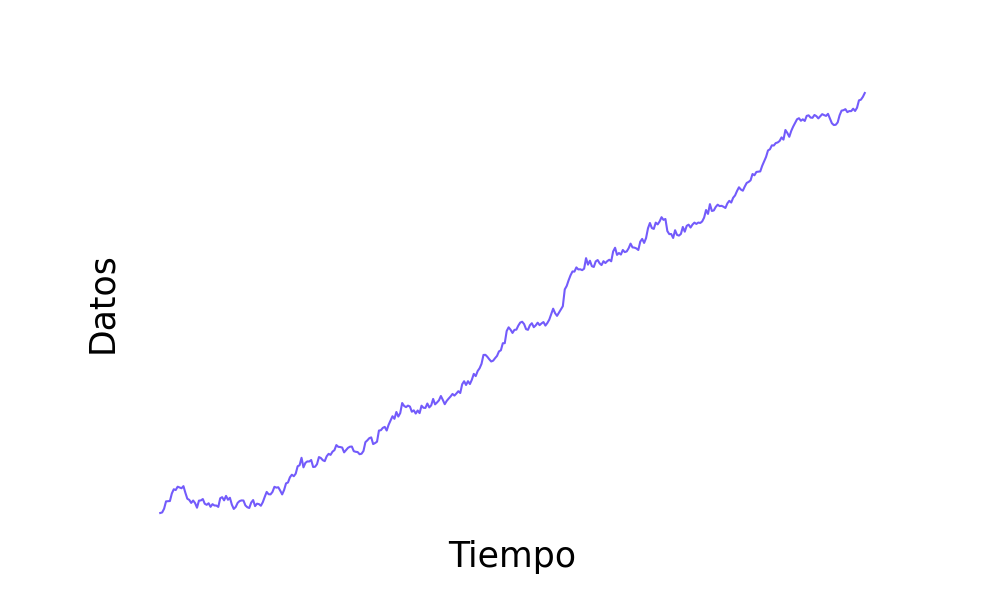
\includegraphics[scale = 0.3]{tendencia}
	\caption{Ejemplo de serie temporal con tendencia ascendente.}
	\label{tend}
\end{figure}


\B{Estacionalidad}

La \B{estacionalidad} es uno o varios patrones recurrentes que ocurren en una serie temporal en periodos de tiempo regulares. La duración de dichos patrones es constante a lo largo del tiempo. 
\begin{figure}[H]
	\centering
	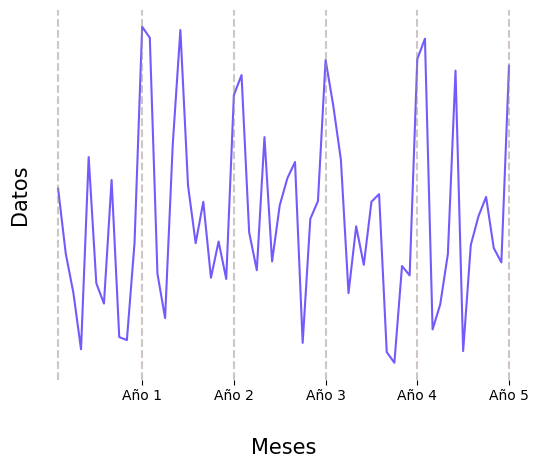
\includegraphics[scale = 0.5]{seasonality}
	\caption{Ejemplo de serie temporal con estacionalidad.}
	\label{estac}
\end{figure}
La serie temporal en la Figura \ref{estac} es estacional porque justo antes del final de cada año ---i.e. periodo regular---, se puede ver una subida repentina en los datos. Además, la duración de estas subidas es constante (en torno a un mes, aproximadamente).

La Figura \ref{estac} también sirve para aclarar que  una serie temporal con  estacionalidad no es lo mismo que una serie temporal periódica. Que sea periódica implica que sea estacional, pero la relación inversa no se cumple.

\B{Ciclos}

Los {\hypertarget{ciclo}{\B{ciclos}} ocurren cuando una serie temporal presenta subidas y bajadas repentinas que no son periódicas y tampoco regulares. Véase la Figura \ref{ciclo}.
	\begin{figure}[H]
		\centering
		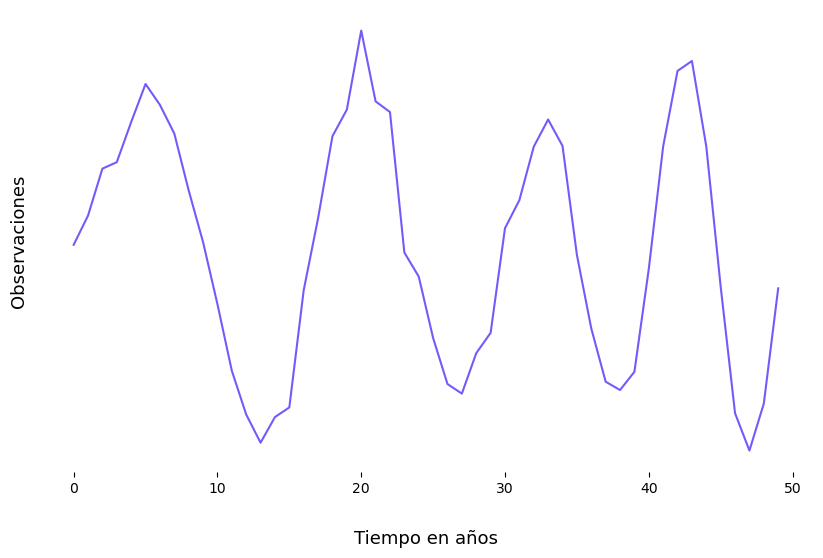
\includegraphics[scale = 0.3]{ciclo}
		\caption{Ejemplo del componente cíclico.}
		\label{ciclo}
	\end{figure}
	
No hay que confundir estacionalidad con patrones cíclicos; no tienen nada que ver: el ciclo no tiene duración fija ni periodicidad. Además, es más impredecible y lo normal es que se supere el año (como mínimo) entre un ciclo y el siguiente.

\bigskip

\B{Residuo}

El residuo (o ruido) es un componente que presentan todas las series temporales. No sigue ningún patrón y por tanto, es impredecible. Véase la Figura \ref{ruido}.

\begin{figure}[H]
	\centering
	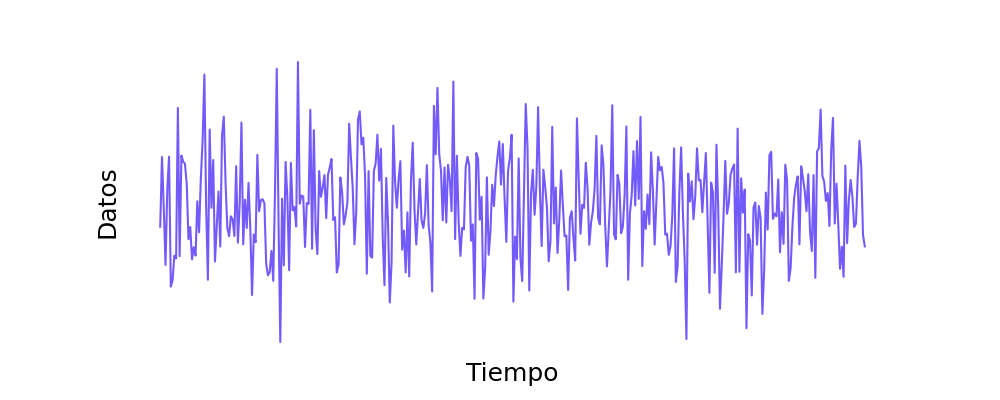
\includegraphics[scale = 0.3]{ruido}
	\caption{Ruido.}
	\label{ruido}
\end{figure}

En el residuo, están recogidos todos aquellos eventos impredecibles como catástrofes, azar, pandemias, etc.

En la Figura \ref{components} se puede ver de una manera más clara cada componente de manera aislada dada una serie temporal\fnm.

\fnt{El componente de ciclo, suele estar incluido en la tendencia. En muchos libros se habla de tendencia-ciclo como una única componente \parencite{otext}, mientras que en otros hacen una clara distinción entre estas dos componentes \parencite{terence} \parencite{brockwell}.}
\begin{figure}[H]
    \centering
    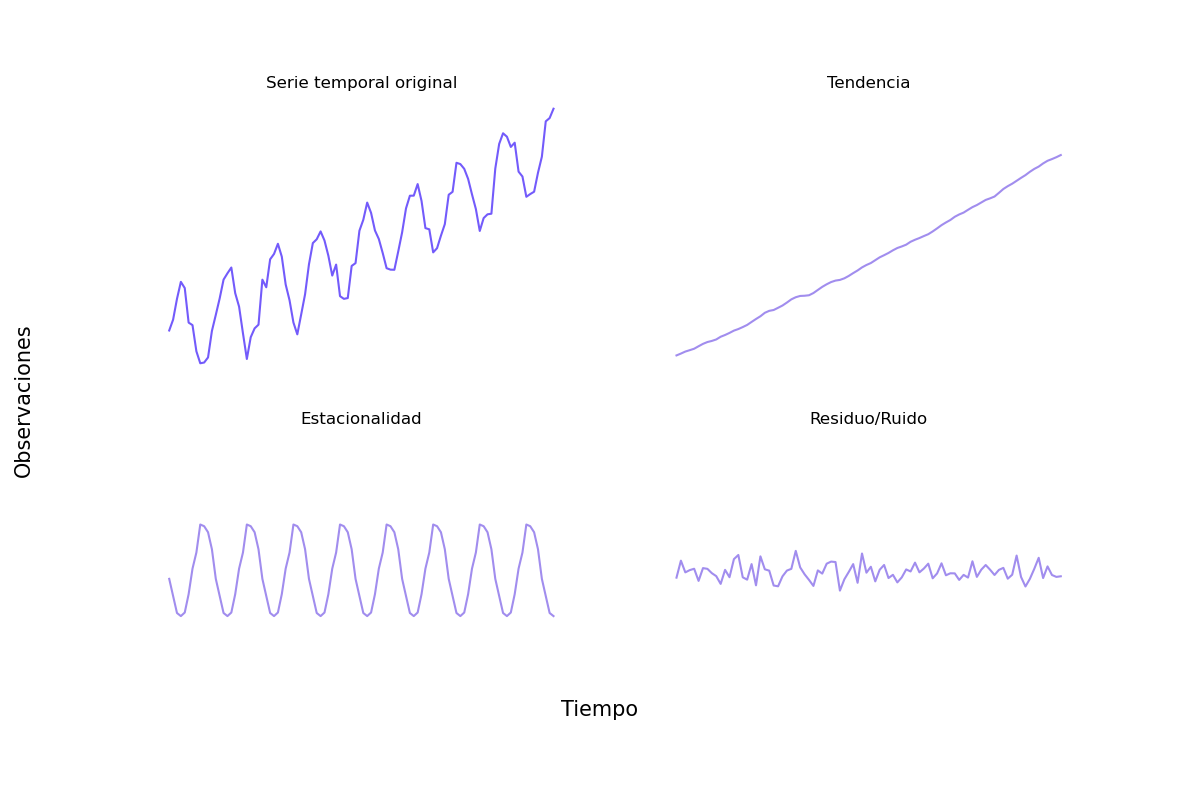
\includegraphics[scale = 0.4]{imgs/componentes.png}
    \caption{Componentes de una serie temporal por separado.}
    \label{components}
\end{figure}
\bigskip

Ahora, tan importante es tener los datos en sí, como conseguir almacenarlos en un lugar seguro y accesible para posteriormente poder procesarlos y visualizarlos. Esto es lo que tratarán los siguientes apartados.

\subsubsubsection{Servicios en la nube}
Mientras que hace no mucho tiempo el almacenamiento de datos era \ti{on-premise} —es decir, dentro de la propia empresa—, en el siglo XXI han surgido nuevas soluciones de almacenamiento en la nube. Los proveedores más importantes de soluciones en la nube son Amazon Web Services de Amazon \parencite{AWS}, Google Cloud Platform de Google \parencite{GoogleCloud} y Azure de Microsoft \parencite{Azure}. Los servicios que principalmente ofrecen estas (y otras) empresas son tres: IaaS (\ti{Infraestructure as a Service}), PaaS (\ti{Platform as a Service}) y SaaS (\ti{Software as a Service}). Estos son los servicios principales y de los que cuelgan otros servicios como DBaaS (\ti{DataBase as a Service}) o STaaS (\ti{Storage as a Service}). Este trabajo en concreto se enfocará en PaaS.

Una de las principales ventajas de contratar servicios en la nube es que uno no se tiene que preocupar ni del mantenimiento, ni de la escalabilidad, ni de las actualizaciones de lo que contrata. PaaS es un término utilizado cuando se contrata un servicio en el que el programador se quiere centrar únicamente en el desarrollo de la aplicación. Es decir, que como ventajas adicionales a las recientemente dichas, en el servicio como plataforma, el desarrollador no se debe de preocupar de la infraestructura que hay por debajo, ni de la configuración a bajo nivel; únicamente de la aplicación que este esté desarrollando.

\subsubsubsection{Visualización de datos}
La visualización de datos es un tema fundamental en el análisis de datos. La necesidad de saber interpretar datos es un tema común en una infinidad de áreas como pueden ser el tiempo, la historia, estadística, deportes, videojuegos, política, finanzas, economía, etc. Y todas aquellas áreas donde esto sea necesario, será vital contar con una o varias visualizaciones que muestren información que desea al público objetivo.

Y es que ser capaz de mostrar en una gráfica la información relevante de una manera clara, sencilla, con los colores adecuados y otros aspectos estéticos importantes es un reto para un ingeniero de datos. Como principales aspectos a tener en cuenta en una visualización están los Principios de Gestalt \parencite{gestalt}, los mecanismos de atención estudiados por la psicóloga Ann Treisman \parencite{treisman} y la teoría y psicología del color.

Los gráficos, además de ser claros y seguir las reglas recién mencionadas, deben tener en cuenta a personas con discapacidades (visuales sobre todo) y deben hablar por sí mismos. Una buena gráfica no necesita que se explique. De esta manera, una visualización sirve como puente de comunicación entre un experto en datos y una persona sin ningún conocimiento en esta área. 

Algo muy característico y muy importante hoy en día es la visualización de datos que todavía no han ocurrido; visualizar predicciones y poder sacar conclusiones acerca de estas para tomar las decisiones adecuadas y anticiparse a los acontecimientos. Para ello, los algoritmos de aprendizaje automático son fundamentales. Estos se van a encargar de estudiar los datos, aprender de ellos (características, patrones, etc.) y proyectar este aprendizaje en el futuro. De esta manera, los algoritmos de aprendizaje automático tratarán de aprender estas componentes para realizar una predicción. Este aprendizaje es fundamental para generar nuevos datos, con las mismas características y patrones en el futuro.


\subsubsection{Aprendizaje automático}

El aprendizaje automático (también conocido como \ti{Machine Learning} en inglés) es una rama de la inteligencia artificial. Esta rama se centra en el diseño de algoritmos matemáticos con el objetivo de que aprendan por sí solos (de ahí el nombre) principalmente a través de errores que cometen en los datos de entrenamiento y experiencia.

Hay tres tipos de aprendizaje automático: aprendizaje supervisado, aprendizaje no supervisado y aprendizaje por refuerzo. Este trabajo, al tratarse de predicción de series temporales, se le proporciona al algoritmo tanto el \ti{timestamp} de un dato como su valor; luego, es un aprendizaje supervisado.

Actualmente, hay numerosos algoritmos disponibles ---y todos ellos sólidos--- que un programador puede emplear para resolver un problema de predicción. De esta manera, en una primera instancia no se sabe cuál va a ser el algoritmo con el que mejores resultados se van a obtener. Es por ello que, es común aplicar varios algoritmos con el fin de poder compararlos y elegir al mejor. Otra puerta que deja abierta el aplicar varios algoritmos para un mismo problema, es lo que se conoce como \ti{bagging}\fnm.


\fnt{\ti{Bagging} es una técnica de aprendizaje automático que consiste en obtener un resultado predictivo final a partir de \ul{promediar} resultados de varios modelos.}

Los algoritmos pues, que se van a emplear en este trabajo son cuatro: XGBoost, LightGBM, Transformer (Informer) y TCN (\ti{Temporal Convolutional Networks}). Todos ellos son muy potentes a día de hoy y se utilizan en numerosas aplicaciones ---no solo en series temporales---. Sin ir más lejos, una de las tecnologías que más popularidad ha ido ganando en los últimos años es el famoso chatbot ChatGP\B{T}. Bien, pues la T en \ti{GPT} es de \ti{\ul{T}ransformer}.

Los modelos generados por estos algoritmos, dado que van a generar nuevos datos en el futuro ---i.e. que no existen---se dice que son \B{modelos generativos}. Esto es debido a otra de las características de las series temporales: su predicción es \B{extrapolar} y no intrapolar\fnm.
\fnt{Esto se explica un poco más en detalle en el \ti{apéndice}\textsuperscript{\hyperref[ap:intravsextra]{A3}}.}

 

Un concepto importante a destacar es la diferencia entre un algoritmo y un modelo ---dos términos que a menudo se usan se emplean indistintamente---. De manera simple, \B{un algoritmo genera un modelo}. En otras palabras, el algoritmo se encarga de aprender las características de los datos y el modelo es la representación de este aprendizaje. 

\bigskip

\B{Gradient Boosting: XGBoost \& LightGBM}

XGBoost y LightGBM no son algoritmos de aprendizaje automático, sino que son bibliotecas de programación que emplean métodos \ti{ensemble}; concretamente \ti{boosting}.

\ti{Ensemble}, en español, significa \B{conjunto}. Métodos \ti{ensemble}, por tanto, es una práctica de aprendizaje automático en la que se aplican varios modelos para obtener una predicción final. Cabe resaltar que cada uno de estos modelos puede haber sido generado por un algoritmo distinto. La filosofía detrás de utilizar métodos \ti{ensemble} está en que varios modelos son capaces de predecir mejor que un único modelo. 

A pesar de que haya varios métodos \ti{ensemble} como \ti{bagging} o \ti{stacking}, XGBoost y LightGBM pertenecen  al método de \B{boosting} (impulso). Este, consiste en generar una regla de decisión final muy precisa, a partir un conjunto de reglas muy simples. En otras palabras,  \ti{boosting} consiste en generar un modelo final muy preciso, a partir una \B{suma ponderada} de modelos simples. 

Un ejemplo donde se puede ver este concepto de manera muy clara es en un problema de clasificación, en el que se trata de clasificar un animal como gato o no gato. Si un modelo muy simple es capaz de detectar, a partir de una imagen, si un animal tiene o no tiene bigotes; otro modelo si tiene orejas puntiagudas; otro modelo si el animal tiene cuatro patas, etc. Al final, el conjunto de estas reglas simples son capaces de generar un modelo final muy preciso. A estos modelos simples se les conoce como \ti{weak learners} o como \ti{base learners}\fnm. Está demostrado que un conjunto de estos son capaces de generar un modelo preciso (\ti{strongly learner}) \parencite{weakLearnStrongLearn}.
\fnt{\ti{Weak learner} o \ti{base learner} es cualquier modelo simple capaz de generar predicciones con algo más de precisión que un modelo aleatorio. Modelo simple, \ti{weak learner} y \ti{base learner} se emplean de manera intercambiable en este trabajo.}

Aunque cada algoritmo de \ti{boosting} sigue sus reglas específicas, el proceso general es el siguiente:
\begin{enumerate}
    \item Se crea un modelo muy simple (\ti{weak learner}).
    \item Se identifican los elementos que se han predicho bien y mal por el modelo.
    \item Se calcula la precisión del modelo.
    \item Se crea otro modelo simple (\ti{weak learner}) que se enfoca en corregir los errores del anterior, y por tanto, mejora la precisión del anterior.
    \item Se repiten pasos 1-4 hasta llegar a una condición de parada como puede ser generar $M$ modelos, alcanzar una precisión requerida, etc.
\end{enumerate}

Uno de los primeros algoritmos más populares de \ti{boosting} fue AdaBoost \parencite{adaBoostTheory} \parencite{adaBoostPract} que asignaba mayores pesos a los datos mal clasificados para que el modelo posterior se centrara más en ellos. Es decir, en AdaBoost, no se elige el siguiente modelo basándose en una función de perdida. Esta manera de enfocar la elección del siguiente modelo (con base en una función de pérdida) fue propuesta no mucho después \parencite{costFunction}. Es a partir de esta idea, que surge el concepto de \ti{Gradient Boosting} (GB) ---también conocido como \ti{Gradient Boosting Machines}  (GBM)--- \parencite{GBM}.

XGBoost significa \ti{Extreme Gradient Boosting} y LightGBM \ti{Light Gradient Boosting Machine}. Es decir, estas dos \B{bibliotecas} (no algoritmos) aplican \ti{Gradient Boosting} (algoritmo) para realizar una predicción final.

\ti{Gradient Boosting} es un método que aporta mucha flexibilidad a la hora de ser empleado. No solo permite al programador elegir entre varias funciones de coste distintas, sino que también permite utilizar varios algoritmos de aprendizaje automático para la generación de modelos. No obstante, debido a sus excelentes resultados, el algoritmo por excelencia empleado por los métodos de \ti{Gradient Boosting} ---y el que emplean XGBoost y LightGBM--- son los árboles de decisión \parencite{CARTwGBM}.

Un árbol de decisión \parencite{CART} consiste en decisiones simples \ti{if-then} respecto a las distintas características de una variable. Estas características se van ramificando con el objetivo de ir segmentando los datos a partir de estas (características). En la Figura \ref{dec_trees} se puede ver un ejemplo simple para predecir las calorías quemadas por una persona dependiendo del tiempo del entrenamiento y su intensidad. 
\begin{figure}[H]
    \centering
    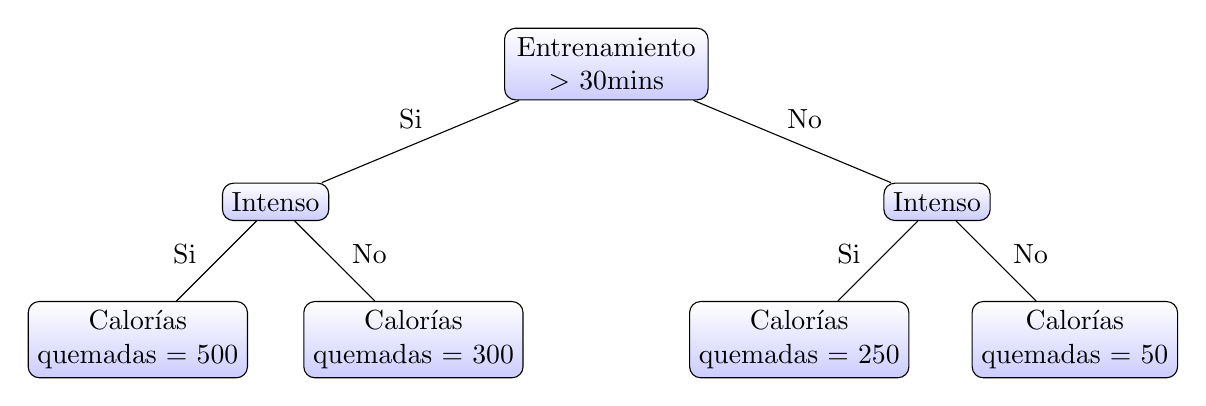
\begin{tikzpicture}[scale = 0.7,
      level distance=2.5cm,
      level 1/.style={sibling distance=12cm},
      level 2/.style={sibling distance=5cm},
      root/.style = {shape=rectangle, rounded corners,
        draw, align=center,
        top color=white, bottom color=blue!20,
        text width=2.35cm
      },
      child/.style = {shape=rectangle, rounded corners,
        draw, align=center,
        top color=white, bottom color=blue!20,
      },
      texto/.style={above, anchor=center} % Apply the 'si' style directly to the node
    ]
        \node[root] {Entrenamiento $>$ 30mins}
        child { node[child] {Intenso} 
          child { node[child] {Calorías \\ quemadas = 500} }
          child { node[child] {Calorías \\ quemadas = 300} }
        }
        child { node[child] {Intenso} 
          child { node[child] {Calorías \\ quemadas = 250} }
          child { node[child] {Calorías \\ quemadas = 50} }
        };
        
        %rama izquierda
        \node[texto] at (-3.55, -1) {Si}; 
        \node[texto] at (-7.65, -3.45) {Si}; 
        \node[texto] at (-4.3, -3.45) {No}; 
        
        %rama derecha
        \node[texto] at (3.6, -1) {No}; 
        \node[texto] at (4.4, -3.45) {Si}; 
        \node[texto] at (7.7, -3.45) {No}; 
    \end{tikzpicture}
    \caption{Ejemplo sencillo aplicando árboles de decisión para un problema de regresión.}
    \label{dec_trees}
\end{figure}

Entrando más en detalle en cómo funciona este método, \ti{Gradient Boosting} hace referencia a aplicar un descenso de \ul{gradiente}\textsuperscript{\hyperref[ap:desc_grad]{A4.1}} respecto a una función de coste, para ir obteniendo \ti{base learners} que vayan reduciendo esta función de coste, y finalmente poder hacer una predicción final con todos ellos. El algoritmo general es el siguiente:

\begin{figure}[H]
    \centering
    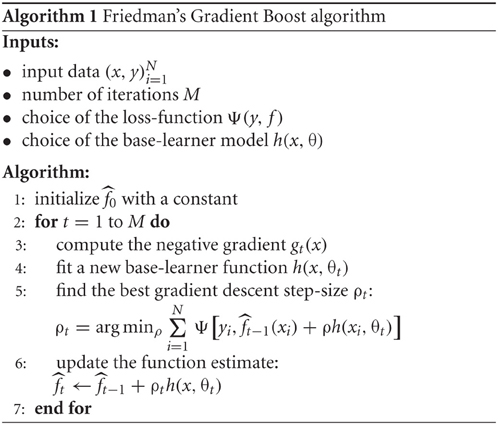
\includegraphics[scale = 0.5]{imgs/GBM_algm.png}
    \caption{Algoritmo de GBM de Friedman. \scriptsize{Fuente: \parencite{GBMtutorial}}}
    \label{GBM_algm}
\end{figure}

El algoritmo de la Figura \ref{GBM_algm} se puede ver como una combinación entre el algoritmo del descenso del gradiente con  los pasos de \ti{boosting} descritos con anterioridad. Consiste en inicializar un modelo inicial $(\widehat{f_0})$ a una constante. Cada modelo que se genere a partir de ahora, se puede interpretar como una función, que depende de unos parámetros (pesos) que genera una salida (resultado del modelo) en base a una función de pérdida\fnm. Esta salida será mejor o peor dependiendo del valor de los parámetros. El número de modelos generados viene determinado por el número de iteraciones $M$, especificadas como entrada en el algoritmo \ref{GBM_algm}. $t$ hace referencia a una iteración en concreto, luego  $t \in [0, M]$.
\fnt{Cabe recalcar que esta interpretación no es específica de \ti{Gradient Boosting}, sino que es aplicable a cualquier algoritmo que genere un modelo.}

Cada uno de estos nuevos modelos generados, se va a tratar de un modelo muy simple (en muchas ocasiones son árboles de un nivel, también conocidos como \ti{tree stump}, véase Figura \ref{simple_gbm_tree}), que tienen como objetivo mejorar de manera leve una función de coste (definida también en la entrada del algoritmo  \ref{GBM_algm}). Este nuevo modelo originado se añade a los que ya se han generado anteriormente. Pero no se añade el modelo completo, sino solo un factor de este, determinado por $\rho$. Este factor determina la distancia a recorrer en dirección contraria al gradiente; o lo que es lo mismo, el grado en que la función de coste se actualiza. Por tanto, es como una tasa de aprendizaje de cada modelo (adicionalmente, luego se aplica una tasa de aprendizaje $\alpha$, también conocido en GBM como \ti{shrinkage}, constante a todos los modelos \parencite{GBM}).

\begin{figure}[H]
    \centering
    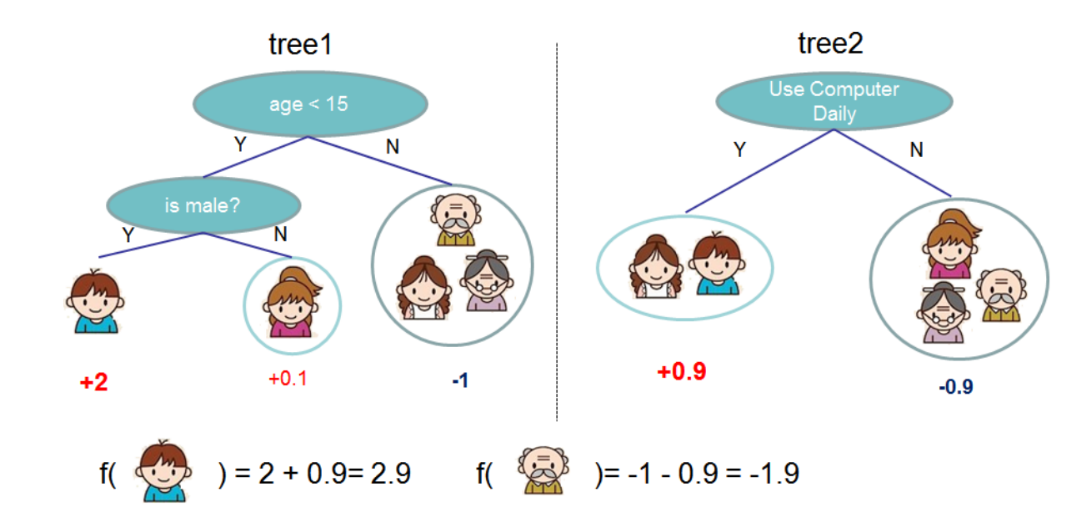
\includegraphics[width = 0.75\textwidth]{imgs/simple_gbm_tree.png}
    \caption{Ejemplo de dos modelos simples de árboles de decisión. Estos modelos se añaden para generar un resultado final. \scriptsize{Fuente: \parencite{XGBoost}}}
    \label{simple_gbm_tree}
\end{figure}
Luego, el resultado de haber aplicado este algoritmo durante $M$ iteraciones, es un modelo final compuesto por $M$ modelos simples capaces de realizar predicciones muy sólidas. Este es el algoritmo detrás de XGBoost y LightGBM. 

\bigskip

\bigskip

\B{XGBoost}

XGBoost \parencite{XGBoost} es una librería que implementa el algoritmo recientemente descrito, pero de una manera muy eficaz. Esto ha provocado que XGBoost sea relativamente común a la hora de ser empleado en competiciones de aprendizaje automático\fnm. Destaca, no solo por los resultados que consigue obtener, sino que también por ser una librería que permite implementar \ti{Gradient Boosting} con las siguientes características:
\fnt{Quizá la más conocida ha sido  \ti{The Netflix Price} \parencite{netflix}}

\begin{itemize}
    \item De manera escalable, siendo capaz de procesar miles de millones de datos.
    \item Es ``paralelizable", lo que supone un aprendizaje más rápido y, por tanto, permite una mayor exploración de modelos (se recuerda que se pueden aplicar varias funciones de coste; luego, esto es importante). Adicionalmente, otras técnicas se emplean para eficiencia.
    \item Se implementa una aproximación del algoritmo \ti{exact greedy algorithm} para mejorar el resultado obtenido por el modelo, haciendo que los árboles de decisiones se dividan de la mejor manera posible.
    \item Robusto ante la falta de datos.
    \item XGBoost es capaz de tratar con \ti{datasets} que son tan grandes, que no caben en la memoria RAM.  A esto se le conoce con el término \ti{out-of-core}, y  lo consigue al dividir el \ti{dataset} en trozos, e ir leyendo dichos trozos de disco según se vayan necesitando. En otras palabras, no se procesa el \ti{dataset} de una sola vez.
    \item Como última característica a destacar de XGBoost es la implementación de \ti{shrinkage} (tasa de aprendizaje en GBM) \parencite{GBM}, regularización L1 y L2\textsuperscript{\hyperref[ap:L1L2sec]{A4.2}} y \ti{column subsampling}  para evitar \ti{overfitting}. Esto es porque, si ya de por sí, los métodos de \ti{boosting} pueden dar problemas de overfitting \parencite{boostingOverfitting}, los árboles de decisión suelen acarrear este mismo problema también \parencite{CARToverfitting}.
\end{itemize}

\bigskip

\bigskip

\B{LightGBM}

Pese a la escalabilidad  y eficiencia que XGBoost ofrece, debido al incremento exponencial en la cantidad de datos en el mundo debido al \ti{Big Data}, nuevas soluciones eran necesarias para tratar cada vez con más datos y más variables de dichos datos. Es por esta razón que surge LightGBM \parencite{lightGBM}. Esta librería también implementa, al igual que XGBoost, GBDT (\ti{Gradient Boosting Decision Trees}). Mejora la eficiencia del algoritmo, acelerando el proceso de entrenamiento en un factor de $\times20$ respecto a anteriores implementaciones de GBDT ---como puede ser  XGBoost---, al mismo tiempo que mantiene prácticamente la misma precisión. Esto es posible al conseguir reducir el número de datos del \ti{dataset}, y el número de variables de dichos datos. Son los algoritmos GOSS (\ti{Gradient-based One-Side Sampling}) y EFB (\ti{Exclusive Feature Bundling}) los encargados de esta tarea.
\begin{itemize}
    \item GOSS, es un algoritmo que permite reducir el número de variables del \ti{dataset} de una manera eficaz y sin perder información. Esto lo consigue al ``eliminar" parte de los datos con un gradiente pequeño asociado. 
    
    De manera simplificada, si un dato tiene un gradiente pequeño asociado, quiere decir que ese dato se ha predicho (considerablemente) bien y se puede eliminar del \ti{dataset}. En otras palabras, no interesa mantenerlo porque no genera mejora en el entrenamiento. En cambio, un dato con un gradiente alto, supone que el algoritmo tenga que aprender a predecirlo mejor y, por tanto, interesa mantenerlo. 
    
    De esta manera, GOSS, a un nivel alto de abstracción, mantiene los datos del \ti{dataset} con un gradiente asociado alto, mientras que descarta aquellos datos con un gradiente asociado bajo (esto supone que la distribución de los datos sea alterada y matemáticas adicionales son implementadas; pero esto va más allá del alcance de este trabajo). Que el gradiente sea alto o bajo es determinado por un umbral.
    
    \item EFB, por el contrario, se encarga de reducir las variables (características) de estos datos. Esto es de suma importancia porque simplifica mucho el \ti{exact greedy algorithm} descrito con anterioridad en XGBoost. Dicho algoritmo (XGBoost), a pesar de que se haga una aproximación, es muy costoso, pues tiene que evaluar la información que aporta cada variable para poder hacer la mejor división de árbol posible.
    
    Esto se puede entender muy bien con el ejemplo de la Figura \ref{dec_trees}. En dicha figura se tratan las variables tiempo de entrenamiento e intensidad para predecir las  calorías quemadas. Supóngase que también estuviesen las variables binarias: casado y con empleo. Aunque puede ser que estas variables puedan tener algún tipo de correlación (leve) con las calorías quemadas por una persona durante un entrenamiento, cabe pensar que las variables tiempo de entrenamiento e intensidad son mucho más representativas. En otras palabras, estas dos últimas variables aportan mucha más información que la de saber si una persona está casada y con trabajo a la hora de predecir sus calorías quemadas en un entrenamiento. 
    
    Por tanto, las primeras divisiones de árbol en los primeros modelos, deberán ser respecto a las variables que más información aporten. Luego, el algoritmo deberá calcular la información que aporta cada variable para determinar la mejor división de árbol posible y, por tanto, \B{cuantas menos variables haya, más rápido será este cálculo}.
    
    Esta reducción de variables se consigue al agrupar (\ti{bundle}) variables que son mutuamente exclusivas, i.e. que rara vez tienen valores distintos de cero al mismo tiempo. Un claro ejemplo de esto es la transformación de variables categóricas en \ti{one-hot encoding}\fnm. Esto aumenta de manera considerable las columnas del \ti{dataset} a pesar de que todas estas variables representan una misma cosa (además de  ser variables mutuamente exclusivas). EFB consigue agrupar todas estas columnas en una sola\fnm, consiguiendo reducir la dimensionalidad del \ti{dataset} al mismo tiempo que se conserva la información.
\end{itemize}

\fnt{Los algoritmos no entienden de texto (i.e. variables categóricas), entienden de números. Entonces, si se tiene la variable \ti{localidad} con valores posibles: Madrid y Barcelona, esta columna de localidad se transforma entonces en dos: una de Madrid y otra de Barcelona. Estas columnas son binarias, y tendrán un 1 si dicha localidad es \ti{True} y 0 de lo contrario. A pesar de ser dos columnas, representan una misma cosa (localidad), y además son, por lo general, mutuamente exclusivas (la localidad o es Madrid o es Barcelona).}
\addtocounter{footnote}{1}
\fnt{Cabe remarcar que este agrupamiento de características no es solo a variables que han sido transformadas a \ti{one-hot encoding}.}

Otra manera de ver estos algoritmos, es que GOSS reduce las filas del \ti{dataset}, mientras que EFB disminuye las columnas. Esto provoca que el entrenamiento sea más \ti{ligero} ---de ahí el nombre de \ul{Light}GBM---.

\bigskip

\B{Redes Neuronales: TCN y Transformers}
\label{rrnn}

Estos algoritmos son algo particulares, pues son redes neuronales (RRNN). Hay tantas, tan variadas ---para distintas áreas--- y se emplean tanto, que tienen su propio campo dentro del aprendizaje automático: \B{aprendizaje profundo} (\ti{Deep Learning}). Véase la Figura \ref{IA}.
\begin{figure}[H]
    \centering
    \resizebox{0.7\textwidth}{!}{%
    \begin{tikzpicture}
        \fill[morados] (0.5,0) ellipse (7.5cm and 4cm);
        \fill[moradmed] (2.5,0) ellipse (5cm and 3cm);
        \fill[moradcl] (4,0) ellipse (3cm and 2cm);
        \node[align=center, font=\large] at (-4.5,0) {Inteligencia\\ artificial};
        \node[align=center, font=\normalsize] at (-0.5,0) {Aprendizaje\\ automático};
        \node[align=center, font=\small] at (4,0) {Aprendizaje\\ profundo};
    \end{tikzpicture}
    }
    \caption{Relación entre inteligencia artificial, aprendizaje automático y aprendizaje profundo.}
    \label{IA}
\end{figure}

El inicio de las redes neuronales se da en 1943, con el primer modelo matemático sugerido de una simple neurona artificial \parencite{artneu}. La base lógica de las redes neuronales se basa en tratar de imitar el comportamiento de las neuronas biológicas en un ordenador. El cerebro ---a un nivel alto de abstracción--- está compuesto por un gran número de neuronas, interconectadas entre sí y recibiendo impulsos de sus conexiones vecinas. Si la suma de estos impulsos supera un umbral, esta neurona emite un impulso eléctrico a sus neuronas vecinas.

Una arquitectura que involucrase más de una neurona artificial y con capacidad de auto-aprendizaje fue introducida en 1958, por el psicólogo Frank Rosenblatt \parencite{perceptrón}. Esta arquitectura, conocida como \B{perceptrón}, consistía únicamente de una capa de entrada y otra de salida. 

Años más tarde, surge la arquitectura MLP (\ti{Multi-layer Perceptron}) \parencite{originsMLP}, con capas ocultas\fnm\ entre la capa de entrada y de salida. Véase la Figura \ref{mlp}.

\fnt{El término \ti{\B{Deep} Learning} viene del gran número de capas ---i.e. profundidad $\rightarrow$ \ti{deep}--- que estas poseen.}
\bigskip

\begin{figure}[H]
	\begin{center}
		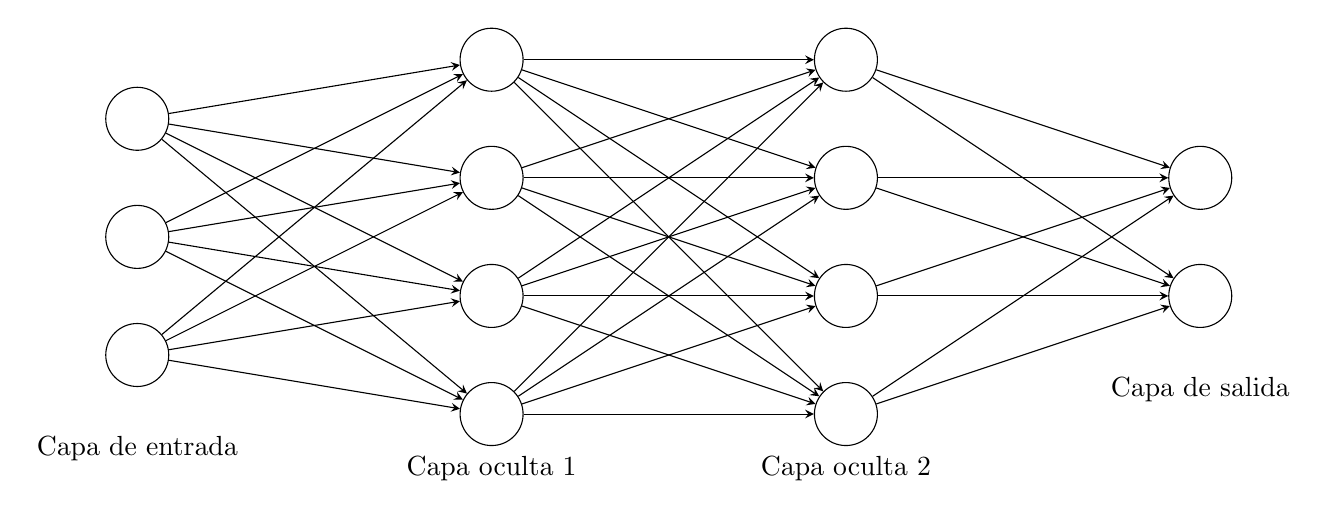
\begin{tikzpicture}[x=1.5cm, y=1.5cm, >=stealth]
			
			% Input layer
			\foreach \i in {1,...,3}
			\node[circle, draw, minimum size=8mm] (input\i) at (0,\i-1) {};
			
			% Hidden layer
			\foreach \i in {1,...,4}
			\node[circle, draw, minimum size=8mm] (hidden1\i) at (3,\i-1.5) {};
			
				\foreach \i in {1,...,4}
			\node[circle, draw, minimum size=8mm] (hidden2\i) at (6,\i-1.5) {};
			
			% Output layer
			\foreach \i in {1,...,2}
			\node[circle, draw, minimum size=8mm] (output\i) at (9,\i-0.5) {};
			
			% Connections Input layer -> Hidden 1 layer
			\foreach \i in {1,...,3}
			\foreach \j in {1,...,4}
			\draw[->] (input\i) -- (hidden1\j);
			
			% Connections Hidden 1 layer -> Hidden 2 layer
			\foreach \i in {1,...,4}
			\foreach \j in {1,...,4}
			\draw[->] (hidden1\i) -- (hidden2\j);
			
			% Connections Hidden 2 layer -> Output layer
			\foreach \i in {1,...,4}
			\foreach \j in {1,...,2}
			\draw[->] (hidden2\i) -- (output\j);
			
			% Labels
			\node[below, yshift=-0.5cm] at (input1.south) {Capa de entrada};
			\node[below] at (hidden11.south) {Capa oculta 1};
			\node[below] at (hidden21.south) {Capa oculta 2};
			\node[below, yshift=-0.5cm] at (output1.south) {Capa de salida};
			
		\end{tikzpicture}
		\caption{Ejemplo arquitectura de un perceptrón multi-capa con dos capas ocultas.}
            \label{mlp}
	\end{center}
        
\end{figure}
Las RRNN se volvieron muy populares gracias al algoritmo de \ti{backpropagation} \parencite{bp} el cual mejoraba la manera en la que estas aprendían. Consiste en propagar hacia atrás los errores cometidos por las neuronas para que estas aprendan \ti{por sí solas}. Esto se consigue al aplicar una función de coste cuyo objetivo es minimizarla lo máximo posible. 

Las MLP dieron lugar a otras redes neuronales, específicas para otras áreas de la inteligencia artificial. Por ejemplo, las RNN (\ti{Recurrent Neural Networks}) \parencite{rnn}\fnm, o  las CNN (\ti{Convolutional Neural Network}) \parencite{cnn}. 

\begin{itemize}
    \item Las RNN, se dice que tienen \ti{memoria}. Se aplican en campos como el procesamiento de lenguaje (NLP), reconocimiento de voz o \B{series temporales}. Sin embargo, estas sufrían de dos problemas principales: el desvanecimiento de gradiente y/o explosión de  gradiente\textsuperscript{\hyperref[ap:grad]{A5}}; y, por otra parte, que no eran capaces de retener memoria a largo plazo. Las LSTM\fnm\ \parencite{lstm} y las GRU\fnm\ \parencite{gru} solventaban estos problemas; y, por ende, obtenían un mejor rendimiento que las RNN \parencite{rnnvslstmgru}.
    \item Las segundas, las CNN,  fueron  un gran avance en el campo de la visión por computador para procesamiento de imágenes. 
\end{itemize} 
\fnt{\ti{Long Short-Term Memory}.}
\addtocounter{footnote}{1}
\fnt{\ti{Gated Recurrent Units}.}
\addtocounter{footnote}{1}
\fnt{Como curiosidad, Michael I. Jordan fue alumno de Rumelhart (uno de los autores del artículo de \ti{backpropagation}). De hecho, en ambos artículos: \parencite{rnn} y \parencite{bp} se mencionan las RNN.}

\bigskip

\B{Transformers: Informer}

\label{sec_informer}

Los Transformer \parencite{transformers}, no son una red neuronal específica de las series temporales, ni mucho menos. De hecho, los Transformer tienen su origen en otro campo: el campo del \B{procesamiento del lenguaje natural} (NLP por sus siglas en inglés). De manera muy resumida, los Transformer sustituyeron a las RNN en esta área al obtener resultados significativamente mayores\fnm.
\fnt{Se deja en el apéndice\textsuperscript{\hyperref[ap:trans]{A6}} más información acerca de los Transformer y qué ventajas suponen frente a RNN; así sobre cómo funcionan y cómo es su arquitectura.}
       
Los Transformer, una de las grandes ventajas que tienen ---y uno de los motivos por los que están establecidos como estado del arte en muchas áreas--- es por su capacidad de aprender \B{distintos contextos} en un \ti{input} (datos). Esto los convierte, \ti{a priori}, en una solución viable para ser aplicados a series temporales. Por poner un ejemplo muy claro donde se ve la necesidad de aprender varios contextos series temporales, es pensando en datos de tráfico. Si estos datos son recogidos cada hora durante un año entero, hay varios contextos (dependencias) que se pueden dar: patrones diarios (hay más tráfico por las mañanas y por las tardes que a medio día y muy de noche); pero también puede haber patrones semanales (el tráfico los fines de semana por la noche es mayor que los días de diario), patrones por vacaciones (salida de Semana Santa) y patrones estacionales/anuales (suele haber menos tráfico en verano, pues la gente está de vacaciones). 

Es la necesidad de aprender estos contextos varios, la razón por la que los Transformer se convierten en una opción más viable a otros algoritmos que suponían el estado del arte hasta entonces \parencite{learnablePosB} como pueden ser: ARIMA\parencite{ARIMA}, LSTM \parencite{lstm}, GRU \parencite{gru} y modelos Seq2Seq con atención \parencite{rnnPlusAttention} .

Otro de los motivos por el cual los Transformer son tan atractivos para las series temporales, es porque su mecanismo de atención le permite al algoritmo aprender relaciones complejas entre \B{datos muy distantes entre sí}. Esto es crucial en series temporales, pues en el ejemplo mencionado recientemente, se ha explicado que puede haber dependencia entre datos entre un año y otro.

Sin embargo, la arquitectura \ti{estándar} de un Transformer, como se ha dicho, fue diseñada para procesamiento de texto y no para datos temporales. Aunque ambos tipos de datos tengan algunos puntos en común, difieren en algunos aspectos que implican que la arquitectura del Transformer original \parencite{transformers} no sirva para series temporales. Se mencionan algunas de estas diferencias:

\begin{itemize}
    \item En una primera instancia, la atención calculada en el Transformer se hace mediante las matrices $Q$ y $K$. Las filas de dichas matrices representan un vector por cada palabra. Esto implica que la complejidad  para  calcular la atención en los Transformer sea exponencial ($\mathcal{O}(L^2$)). Luego, añadir un nuevo dato a la secuencia ($L$)---ya sea texto, serie temporal, etc.--- incrementa de manera exponencial la complejidad del algoritmo ---lo que lo convierte en una vía poco viable para secuencias de  datos muy largas---. Esto, aunque suponga un problema para secuencias largas (independientemente de si es texto, series temporales, etc.), si es cierto que el texto, no solo se puede dividir de una manera más sencilla ---e.g. en párrafos que no tengan relación entre sí---, sino que también su secuencia tiende a ser bastante más corta que la de una serie temporal\fnm. Además, la dependencia entre datos (palabras) muy distanciadas entre sí no es tan extrema como en series temporales. Esto se traduce en que \B{la manera de calcular la atención del Transformer original sea inviable para series temporales} \parencite{surveyTransfTS}.
    \fnt{Se puede pensar en las preguntas que se le hacen a ChatGPT; de media, suelen ser pocas palabras respecto a los cientos y miles de datos que suelen formar una serie temporal.}
    \addtocounter{footnote}{1}
    \fnt{En el ejemplo de tráfico mencionado anteriormente, datos recopilados cada hora, pueden tener relación con datos de hace un año, i.e. con datos a una distancia de $365\times24 = 8760$ periodos. Un texto, normalmente dividido en palabras, muy difícil es que una palabra necesite el contexto de otra a tanta distancia.}
    \item Otra diferencia a destacar entre texto y series temporales es la \B{importancia del contexto local} en esta última. Es decir, en series temporales son muy importantes los patrones, i.e. formas en la gráfica que se repiten en cierta ventana periodo de tiempo. Mientras que el Transformer original dispone de \ti{MultiHead Attention} para capturar múltiples contextos, puede no ser suficiente al no indicarle explícitamente la importancia del contexto local. Es por esto que es importante que la atención del Transformer se enfoque especialmente en datos cercanos a uno dado para poder capturar las formas de la serie temporal ---i.e. contexto local---. Véase la Figura \ref{local_context}.
    \begin{figure}[H]
        \centering
        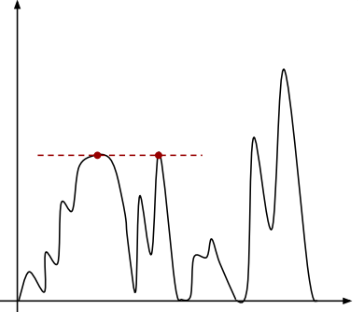
\includegraphics[width = 0.25\textwidth]{imgs/local_cont1.png}
        \hspace{2.5cm}
        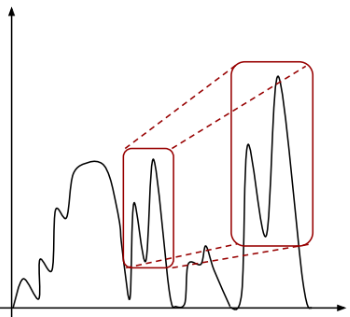
\includegraphics[width = 0.25\textwidth]{imgs/local_cont2.png}
        \caption{Mientras que la atención del Transformer original puede asignar una alta dependencia entre los dos datos señalados en la figura de la izquierda, una atención local puede percibir mejor las formas de la serie temporal (figura de la derecha). \scriptsize{Fuente: \parencite{logSparse}}}
        \label{local_context}
    \end{figure}

    \item Aunque los autores del Transformer \parencite{transformers}, afirmen que sus resultados con un codificador de posicionamiento fijo (\ti{fixed}) ---senos y cosenos--- se obtienen resultados muy similares a los de emplear un codificador de posicionamiento \ref{distill} ``aprendible" (\ti{learnable)} \parencite{learnableOverFixed1}, estudios posteriores \parencite{learnableOverFixed2} han demostrado que el segundo es generalmente mejor; sobre todo para series temporales \parencite{learnablePosB}.
\end{itemize} 

\fnt{Se puede pensar en las preguntas que se le hacen a ChatGPT; de media, suelen ser pocas palabras respecto a los cientos y miles de datos que suelen formar una serie temporal.}

Pese a que las primeras modificaciones realizadas a la arquitectura del Transformer para aplicarlas a series temporales tenían en cuenta estos puntos \parencite{SparseTransformer}, \parencite{logSparse},  el \B{Informer} \parencite{informer} va un paso más allá añadiendo ciertas modificaciones extra  que mejoraron los resultados obtenidos hasta la fecha.

El Informer introdujo cuatro nuevos cambios:
\begin{itemize}
    \item El primero, es que emplea una codificación de posicionamiento relativo, pero \ti{especial}. Y es que, el orden de los datos en una serie temporal es mucho más importante que un texto. No solo porque en un texto se pueden cambiar el orden de las palabras sin alterar el significado de la frase ---e.g. \ti{\ul{coloca la silla} \ul{a la derecha}}--- sino que además el posicionamiento en una serie temporal conlleva un \ti{timestamp}. Este, aporta información adicional ---segundo, minuto, hora, día, etc--- al Transformer y por ello es conveniente tenerlo en cuenta para la predicción. Con esta codificación, el Informer consigue implementar los dos puntos recientemente mencionados: contexto local y codificación ``aprendible''\fnm.
    \item El segundo cambio tiene que ver con reducir la complejidad de atención, haciendo que cada punto de la serie temporal preste atención solo a algunos otros ---y no a todos---. Esto se hace con el algoritmo \ti{ProbSparse self-attention}\fnm. La manera en la que este algoritmo calcula los datos a los que cada punto debe prestar atención tiene mejores propiedades matemáticas que los métodos empleados por los dos anteriores \parencite{SparseTransformer} \parencite{logSparse}. Con esto, se consigue reducir la complejidad de atención a $\mathcal{O}(L \ln L$).
    
    \item El tercer cambio es que, a diferencia del Transformer original, en el que la dimensión de entrada y  salida entre capa y capa ---tanto en el \ti{Encoder} como en el \ti{Decoder}--- era constante siempre. Informer, consigue ir comprimiendo la información para reducir tanto la dimensión de las matrices de salida a la mitad\fnm \hspace{1.5pt} (véase la Figura \ref{maxPooling}) como para ir reduciendo la dimensión de estas capas ---i.e.  números de estas matrices, $h$ en el Transformer original (véase la Figura \ref{distill})---. El objetivo de todo esto es reducir la memoria del algoritmo y reducir aún más ---junto con \ti{ProbSparse self-attention}--- el coste computacional sin perder información relevante.
    \item Como última mejora, Informer hace que el proceso  de predicción del \ti{Decoder}, en vez de ser secuencial, se haga de una sola vez. Esto, con el objetivo que evitar errores acumulados que suceden en las predicciones  secuenciales (véase la Figura \ref{distill}).
\end{itemize}
\fnt{Se deja en el \ti{apéndice}\textsuperscript{\hyperref[ap:codif]{A7.1}} más información sobre la codificación que realiza el Informer en los datos de la serie temporal.}
\addtocounter{footnote}{1}
\fnt{Se deja en el \ti{apéndice}\textsuperscript{\hyperref[ap:prob]{A7.2}} una breve explicación del este algoritmo.}
\addtocounter{footnote}{1}
\fnt{Esto se consigue con un MaxPooling de $2\times2$.}
Véase a continuación la arquitectura del algoritmo y lo explicado recientemente.

\begin{figure}[H]
    \centering
    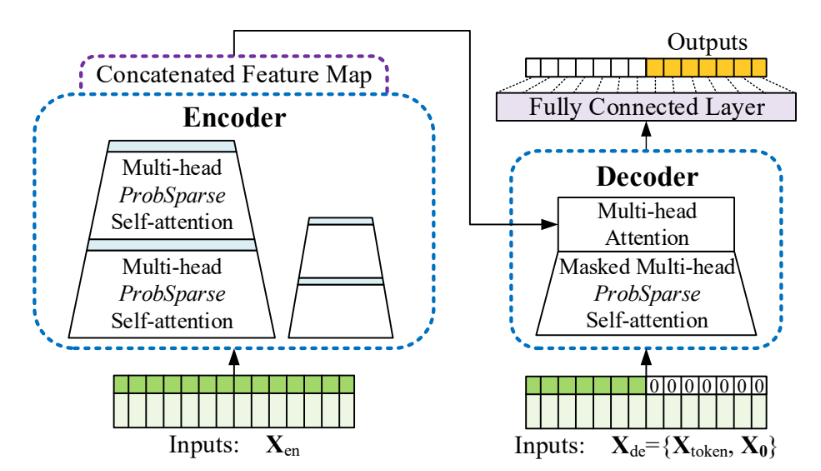
\includegraphics[scale = 0.55]{imgs/informer_distill.png}
    \caption{Arquitectura Informer.  \scriptsize{Fuente: \parencite{informer}}}
    \label{distill}
    % NO CAMBIARLO DE POSICIÓN 
    \begin{tikzpicture}[overlay]
        \draw[black, ultra thick] (-1.7, 2.73)  rectangle (-0.61, 2.012);
        \draw[->, black, ultra thick] (-0.3, 2.35) -- (0.9, 2.35);
        \draw[->, bend right=65, thick] (4.5,2.35) to (4.5,6.25);
    \end{tikzpicture}
\end{figure}
\fnt{$n$ es un hiperparámetro, i.e. se puede elegir.}

En la Figura \ref{distill}, nótese la forma de pirámide, indicando la reducción de dimensiones ($h$) en cada capa (el flujo es hacia arriba). También, nótese como el \ti{Decoder} recibe como entrada los últimos $n$ datos de la serie temporal\protect\fnm\ ($X_{token}$) concatenado con un vector de todos ceros ($X_0$). Este vector $X_0$, su dimensión, representa la cantidad de puntos a predecir en el futuro por el Informer.

\begin{figure}[H]
    \centering
    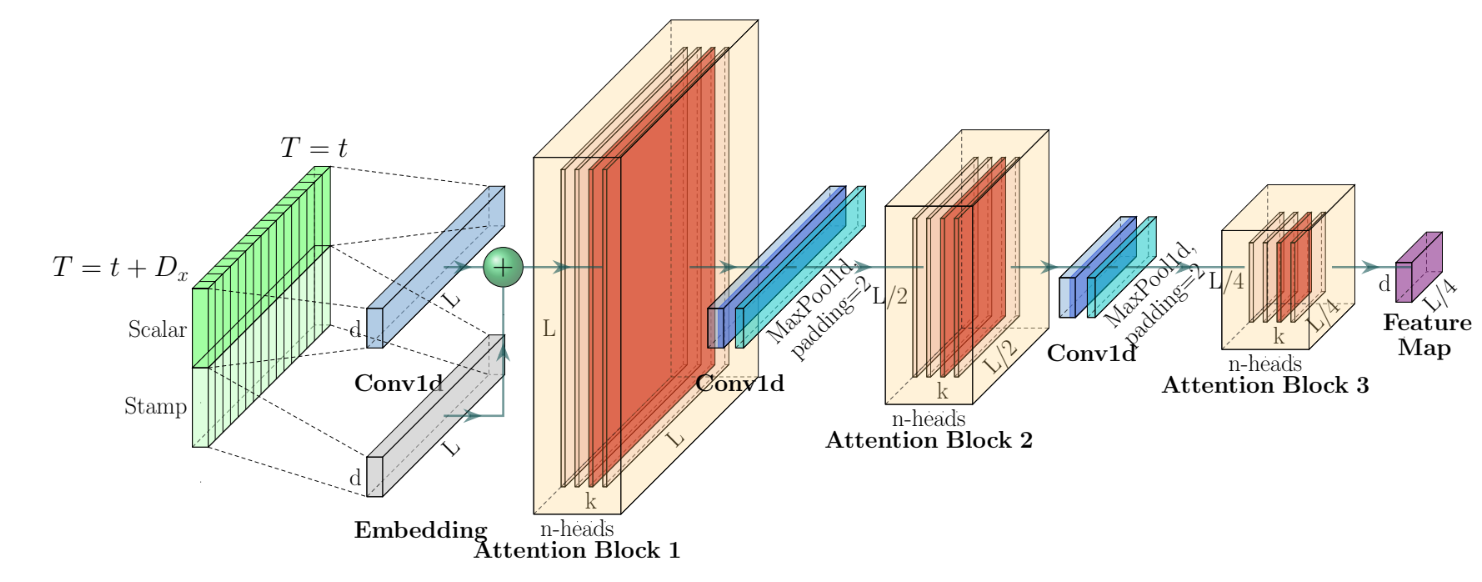
\includegraphics[scale = 0.5]{imgs/informer_maxPooling.png}
    \caption{Input y tres primeras capas del Encoder en el Informer. Nótese cómo se va reduciendo la dimensionalidad ($L$) de las capas de atención (rojo) a la mitad. Esto se consigue con un MaxPooling de $2\times2$. \scriptsize{Fuente: \parencite{informer}}}
    \label{maxPooling}
\end{figure}

Adicionalmente, se deja en el \ti{apéndice}\textsuperscript{\hyperref[ap:inf_res]{A7.3}} una tabla comparativa de este algoritmo con respecto a los que eran el estado del arte hasta el momento.


\B{TCN}

Las TCN (\ti{Temporal Convolutional Networks} \parencite{TCNSeq} se dan en un contexto similar al de los Transformer. Sus autores, también conscientes de los problemas de las RNN comentados  en la sección anterior (secuenciales,  gradiente inestable, memoria, etc.), decidieron crear un algoritmo para la predicción de secuencias\fnm. 

Algo que cabe remarcar, es que no se debe confundir con la otra TCN \parencite{TCNOrig} que se aplican para la segmentación de imágenes. Por tanto, siempre que se mencione el algoritmo TCN en este trabajo, se estará haciendo referencia al algoritmo de secuencias \parencite{TCNSeq}.

Lo particular y diferente de este algoritmo, es que emplea la operación de \B{convolución} para realizar la predicción. Véase la Figura \ref{convol}.
\fnt{Aunque el nombre del algoritmo pueda incitar a pensar que es un algoritmo para series temporales, no es así; es para secuencias. Esto engloba muchos más campos que las series temporales.}

\begin{figure}[H]
    \centering
    \hspace*{-1cm}
    \begin{tikzpicture}[>=Stealth, scale=0.8]
    
        % Input vector
        \foreach \x/\val in {0/{$x_0$}, 1/{$x_1$}, 2/{$x_2$}, 3/{$x_3$}, 4/{$x_4$}} {
            \draw (\x,0) rectangle ++(1,1) node[pos=.5] {\val};
        }
        
        % Convolution kernel
        \foreach \x/\val in {0/{$k_0$}, 1/{$k_1$}, 2/{$k_2$}} {
            \draw (\x,2.5) rectangle ++(1,1) node[pos=.5] {\val};
        }
        
        % Output vector
        \foreach \x/\val in {1/{$y_0$}, 2/{}, 3/{}} {
            \draw (\x,5) rectangle ++(1,1) node[pos=.5] {\val};
        }
        
        % Arrow for convolution
        \draw[->, thick] (2.5,1) -- (2.5,2.5) node[midway, left] {$\times$};
        \draw[->, thick] (1.5,1) -- (1.5,2.5) node[midway, left] {$\times$};
        \draw[->, thick] (0.5,1) -- (0.5,2.5) node[midway, left] {$\times$};
        
        % Arrow for result
        \draw[->, thick] (0.5,3.5) -- (1.5,5);
        \draw[->, thick] (1.5,3.5) -- (1.5,5);
        \draw[->, thick] (2.5,3.5) -- (1.5,5);

        \node[ultra thick, black] at (1.2, 4) {+};
        \node[ultra thick, black] at (1.8, 4) {+};
        
        % Dots for convolution kernel
        \draw (3.5, 3) node[right] {$\text{Kernel} \quad k=3$};
        \draw (5.5, 0.5) node[right] {Input};
        \draw (4.5, 5.5) node[right] {Output};
        
        %##################################
        \hspace{2cm}
        
        % Repetición a la derecha
        \begin{scope}[shift={(7,0)}]
        % Input vector
        \foreach \x/\val in {0/{$x_0$}, 1/{$x_1$}, 2/{$x_2$}, 3/{$x_3$}, 4/{$x_4$}} {
            \draw (\x,0) rectangle ++(1,1) node[pos=.5] {\val};
        }
        
        % Convolution kernel
        \foreach \x/\val in {2/{$k_0$}, 3/{$k_1$}, 4/{$k_2$}} {
            \draw (\x,2.5) rectangle ++(1,1) node[pos=.5] {\val};
        }
        
        % Output vector
        \foreach \x/\val in {1/{$y_0$}, 2/{$y_1$}, 3/{$y_2$}} {
            \draw (\x,5) rectangle ++(1,1) node[pos=.5] {\val};
        }
        
        % Arrow for convolution
        \draw[->, thick] (2.5,1) -- (2.5,2.5) node[midway, left] {$\times$};
        \draw[->, thick] (3.5,1) -- (3.5,2.5) node[midway, left] {$\times$};
        \draw[->, thick] (4.5,1) -- (4.5,2.5) node[midway, left] {$\times$};
        
        % Arrow for result
        \draw[->, thick] (2.5,3.5) -- (3.5,5);
        \draw[->, thick] (3.5,3.5) -- (3.5,5);
        \draw[->, thick] (4.5,3.5) -- (3.5,5);

        \node[ultra thick, black] at (3.2, 4) {+};
        \node[ultra thick, black] at (3.8, 4) {+};
        
        % Dots for convolution kernel
        \draw (6, 3) node[right] {$\text{Kernel} \quad k=3$};
        \draw (5.5, 0.5) node[right] {Input};
        \draw (4.5, 5.5) node[right] {Output};
        \end{scope}
    \end{tikzpicture}
    \caption{Ejemplo entre una secuencia input y cómo se obtiene la secuencia de output a través de la operación de convolución.}
    \label{convol}
\end{figure}

En la Figura \ref{convol} se emplea un \ti{kernel} de tamaño $k = 3$ y se hace la suposición de que la secuencia de entrada es un vector unidimensional\fnm.
\fnt{Podría darse el caso de que la entrada tuviera varios canales. Por ejemplos, una imagen de color es tridimensional. En los ejemplos siguientes se va a suponer que la entrada tiene un canal, es decir, la entrada es un vector unidimensional.}



Las TCN son capaces de mantener relaciones entre datos muy distantes entre sí. Es decir, tienen sustancialmente más memoria que las RNN y su familia (LSTM, GRU, RNN encoder-decoder, etc.). Adicionalmente, son ``paralelizables" y sus gradientes son más estables ---al igual que los Transformer---. Tienen dos características principales, aunque como se comentará más adelante, no son suficientes. Estas características son:
\begin{itemize}
    \item La longitud de secuencia de entrada y de salida coinciden.
    \item No se usa información futura en la predicción de la secuencia. Es decir, dada una entrada de datos $x_0, \cdots, x_t$, y se quiere predecir una secuencia de salida $y_0, \cdots, y_t$, para la predicción de una dato $y_i$ con $i \in [0,t]$ no se usa información de un dato $x_j \hspace{2pt}|\hspace{4pt} j >i$. Esta idea es la misma que la de enmascarar la información en el \ti{Decoder} de los Transformer.
\end{itemize}

En la Figura \ref{convol}  no se cumplen las dos propiedades que recién se han comentado. La dimensión de entrada ($X \in \mathbb{R}^5$) no es la misma que la de salida ($Y \in \mathbb{R}^3$). Y también, para el cálculo de $y_0$, por ejemplo, se han utilizado datos futuros ($x_1$ y $x_2$). Lo mismo para $y_1$ e $y_2$. Para solventar ambos problemas basta con añadir lo que se conoce como \ti{(left) zero-padding}. En este caso, de dos dimensiones ---i.e.  $k-1$---, pero más adelante se verá que cambia. Véase la Figura \ref{tcn2}.

\begin{figure}[H]
	\centering
	\hspace*{-2cm} % Adjust this value to move the figure to the left
	\begin{tikzpicture}[>=Stealth, scale=0.8, shift={(-5cm,0)}]  % Positive shift
		
		% Input vector
		\foreach \x/\val in {-2/{$0$}, -1/{$0$}, 0/{$x_0$}, 1/{$x_1$}, 2/{$x_2$}, 3/{$x_3$}, 4/{$x_4$}} {
			\ifnum\x<0
			\draw[fill=gray!30] (\x,0) rectangle ++(1,1) node[pos=.5] {\val};
			\else
			\draw (\x,0) rectangle ++(1,1) node[pos=.5] {\val};
			\fi
		}
		
		% Output kernel
		\foreach \x/\val in {-1/{$y_0$}, 0/{$y_1$}, 1/{$y_2$}, 2/{$y_3$}, 3/{$y_4$}} {
			\draw (\x,2.5) rectangle ++(1,1) node[pos=.5] {\val};
		}
		
		% Arrow for result
		\draw[->] (-1.5,1) -- (-0.5,2.5) node[midway, right] {};
		\draw[->,] (-0.5,1) -- (-0.5,2.5) node[midway, right] {};
		\draw[->] (0.5,1) -- (-0.5,2.5) node[midway, right] {};
		
		\draw (5, 0.5) node[right] {Input};
		\draw (4, 3) node[right] {Output};
		
		%################################## DERECHA #########################
		\hspace{2cm}  % Adjusted spacing (optional for more space)
		
		% Repetición a la derecha
		\begin{scope}[shift={(7,0)}]
			% Input vector
			\foreach \x/\val in {-2/{$0$}, -1/{$0$}, 0/{$x_0$}, 1/{$x_1$}, 2/{$x_2$}, 3/{$x_3$}, 4/{$x_4$}} {
				\ifnum\x<0
				\draw[fill=gray!30] (\x,0) rectangle ++(1,1) node[pos=.5] {\val};
				\else
				\draw (\x,0) rectangle ++(1,1) node[pos=.5] {\val};
				\fi
			}
			
			% Output kernel
			\foreach \x/\val in {-1/{$y_0$}, 0/{$y_1$}, 1/{$y_2$}, 2/{$y_3$}, 3/{$y_4$}} {
				\draw (\x,2.5) rectangle ++(1,1) node[pos=.5] {\val};
			}
			
			% Arrow for result
			\draw[->] (2.5,1) -- (3.5,2.5) node[midway, right] {};
			\draw[->] (3.5,1) -- (3.5,2.5) node[midway, right] {};
			\draw[->] (4.5,1) -- (3.5,2.5) node[midway, right] {};
			
			\draw (5, 0.5) node[right] {Input};
			\draw (4, 3) node[right] {Output};
		\end{scope}
	\end{tikzpicture}
	\caption{Convolución con zero-padding. Se obvia la convolución para hacerlo más claro.}
	\label{tcn2}
\end{figure}


De esta manera, ya se cumplen las dos primeras características mencionadas anteriormente. A este tipo de convolución se le conoce como \B{convolución causal}. Sin embargo, esto, como ya se ha dicho, no es suficiente. En el apartado anterior de los Transformer, se comentó que los datos temporales pueden tener relación con datos muy distanciados entre sí. Es decir, una propiedad deseable a tener por el algoritmo, es que un punto $y_i$ sea capaz de tener información de $x_0, x_1, \cdots, x_i$, i.e. contexto global. El procedimiento que se está siguiendo, a medida que se van aumentando las capas, no es viable. Véase la Figura \ref{tcn3}.
\begin{figure}[H]
    \centering
    \begin{tikzpicture}[>=Stealth, scale=0.8]
    
        % Input vector
       \foreach \x/\val in {-6, -5, -4/{$x_0$}, -3/{$ $}, -2/{$ $}, -1/{$ $}, 0/{$x_0$}, 1, 2, 3, 4} {
            \ifnum\x<-4
                \draw[fill=gray!30] (\x,0) rectangle ++(1,1) node[pos=.5] {};
            \else
                \ifnum\x<0
                    \draw (\x,0) rectangle ++(1,1) node[pos=.5] {\val};
                \else
                    \draw[fill=moradcl] (\x,0) rectangle ++(1,1) node[pos=.5] {};
                \fi
            \fi
        } 
        \foreach \y/\val in {-3, -2, -1, 0, 1, 2, 3} {
            \ifnum\y<-1
                \draw[fill=gray!30] (\y,2.5) rectangle ++(1,1) node[pos=.5] {};
            \else
                \ifnum\y>0
                    \draw[fill=moradcl] (\y,2.5) rectangle ++(1,1) node[pos=.5] {};
                \else
                    \draw (\y,2.5) rectangle ++(1,1) node[pos=.5] {};
                \fi
            \fi
        }
       
        \foreach \z/\val in {-2, -1, 0, 1, 2/{$y_t$}} {
        \ifnum\z<2
            \draw (\z,5) rectangle ++(1,1) node[pos=.5] {};
        \else
            \draw (\z,5) rectangle ++(1,1) node[pos=.5] {\val};
        \fi
        }
        
        % Arrow for result
        \draw[->] (0.5,1) -- (1.5,2.5) node[midway, right] {};
        \draw[->,] (1.5,1) -- (1.5,2.5) node[midway, right] {};
        \draw[->] (2.5,1) -- (1.5,2.5) node[midway, right] {};

        \draw[->] (1.5,1) -- (2.5,2.5) node[midway, right] {};
        \draw[->,] (2.5,1) -- (2.5,2.5) node[midway, right] {};
        \draw[->] (3.5,1) -- (2.5,2.5) node[midway, right] {};

        \draw[->] (2.5,1) -- (3.5,2.5) node[midway, right] {};
        \draw[->,] (3.5,1) -- (3.5,2.5) node[midway, right] {};
        \draw[->] (4.5,1) -- (3.5,2.5) node[midway, right] {};

        \draw[->] (1.5,3.5) -- (2.5,5) node[midway, right] {};
        \draw[->,] (2.5,3.5) -- (2.5,5) node[midway, right] {};
        \draw[->] (3.5,3.5) -- (2.5,5) node[midway, right] {};
    
        \draw (5, 0.5) node[right] {Input};
        \draw(4, 3) node [right] {Capa 1};
        \draw (3, 5.5) node[right] {Output};
    \end{tikzpicture}
    \caption{Ejemplo de inviabilidad al aumentar capas.}
    \label{tcn3}
\end{figure}

En la Figura \ref{tcn3} se puede ver claramente, que si la entrada fueran cientos de datos, muchas capas intermedias iban a ser necesarias para que la información de $x_0$ le llegue a $y_t$. Esto es porque el campo receptivo entre capa y capa crece de manera lineal. 

Para solventar esto, se introduce el concepto de \B{dilatación} \parencite{waveNet}. Esto quiere decir que, según se van aumentando las capas, el campo receptivo se va expandiendo de una manera exponencial. Una forma muy común de establecer esta dilatación $d$ es a través de elegir una base $b = 2$ y elevarla a $i$: siendo $i$ en número de capas en que esté operando la dilatación. De esta manera, $d = b^i$.  Véase la Figura \ref{tcn4}.

\begin{figure}[H]
    \centering
    \hspace{-3cm}
    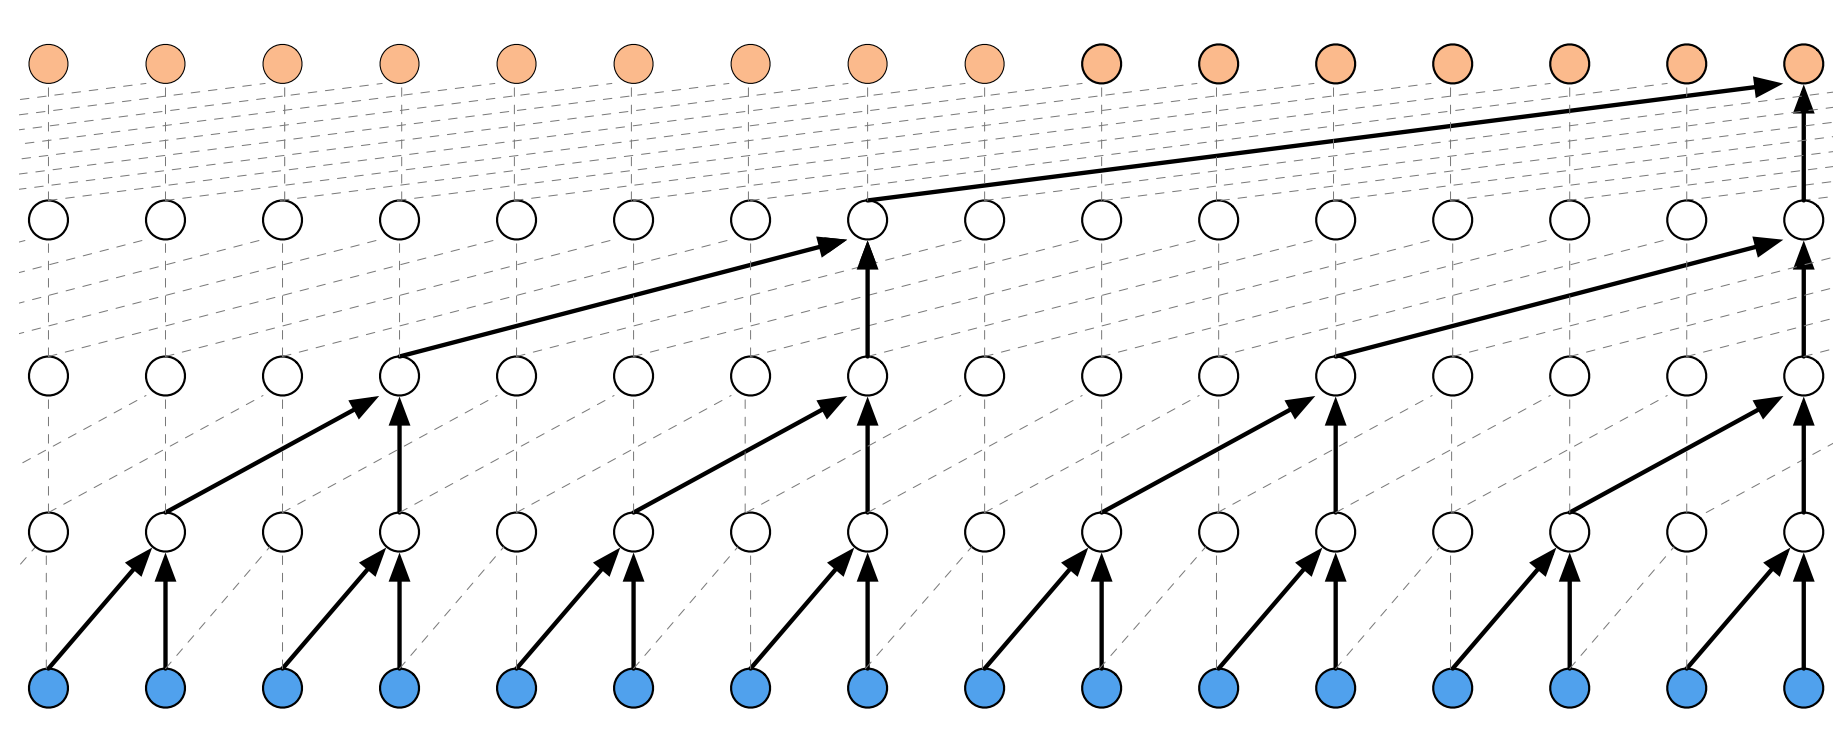
\includegraphics[scale = 0.3]{tcn4}
    \begin{tikzpicture}[overlay]
        \node at (2,0.25) {\footnotesize{Capa $i= 0$: $d = b^0 = 1$}};
        \node at (2,1.25) {\footnotesize{Capa $i= 1$: $d = b^1 = 2$}};
        \node at (2,2.25) {\footnotesize{Capa $i= 2$: $d = b^2 = 4$}};
        \node at (2,3.25) {\footnotesize{Capa $i= 3$: $d = b^3 = 8$}};
    \end{tikzpicture}
    \caption{Dilatación. \scriptsize{Fuente: \parencite{waveNet}}}
    \label{tcn4}
\end{figure}

Cabe remarcar que no cualquier valor de $b$ es válido y compatible con el tamaño del \ti{kernel} $k$ \parencite{TCNpost}. También, la introducción de la dilatación hace que el \ti{(left) zero-padding} ya no sea constante.

Por último, debido a la gran profundidad de la red neuronal, se emplea un bloque residual por capa. Este bloque residual \parencite{bloqueResidual} tiene la misma finalidad que el visto en los Transformer: mejorar la eficiencia del algoritmo. No obstante, es algo distinto. Véase la Figura \ref{tcn5}.

\begin{figure}[H]
    \centering
    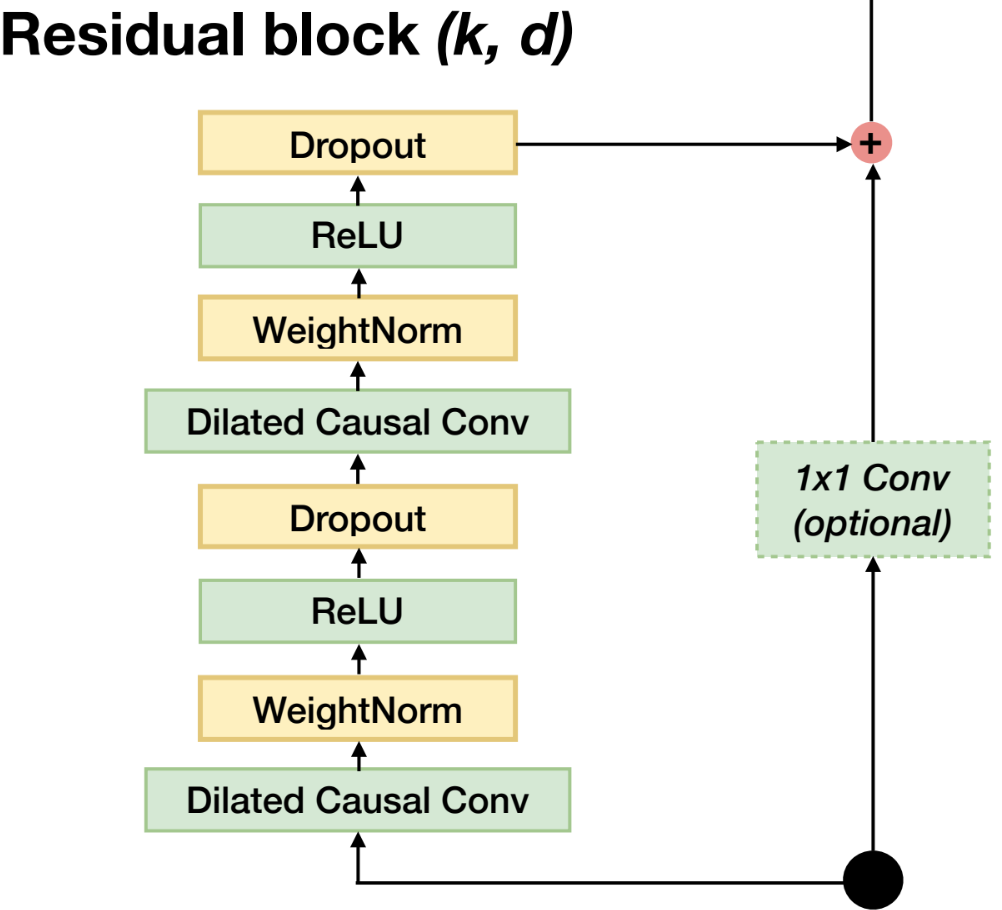
\includegraphics[scale = 0.35]{imgs/tcn5.png}
    \begin{tikzpicture}[overlay]
        \node[left] at (-7,0.8) {\footnotesize{$1^\text{era}$} convolución};
        \node[left] at (-7, 3.7) {\footnotesize{$2^\text{nda}$} convolución};

    \end{tikzpicture}
    \caption{Bloque Residual TCN. \scriptsize{Fuente: \parencite{TCNSeq}}}
    \label{tcn5}
\end{figure}

Es decir, si antes (Figura \ref{tcn4}), en cada capa $i$, se aplicaba una convolución con un tamaño de \ti{kernel} $k = 3$ y una dilatación $d$, ahora se aplican dos. Además, después de cada convolución, se aplica una normalización de los datos \parencite{weightNormalization}\fnm\ para simplificar los valores con los que la red entrena y, por tanto, reducir la complejidad de los cálculos; lo que implica mayor rapidez de entrenamiento. 

Después, se aplica una función de activación ReLu \parencite{ReLu}, para introducir no linealidad a los datos y que la TCN sea capaz de aprender patrones más complejos. Además, como medida para evitar \ti{overfitting}\fnm\ se aplica la técnica de \ti{Dropout} \parencite{dropout}. Esto último, desactiva aleatoriamente neuronas en cada capa, con el fin de que la neurona sea más robusta en el aprendizaje. Por último, el bloque residual suma el \ti{input} de la  capa con el \ti{output} obtenido después de haber hecho todo el proceso. Opcionalmente, en caso de que la entrada no tenga el mismo número de canales (dimensión) que la salida, se aplica un \ti{kernel} para igualar ambas dimensiones y, por tanto, que se puedan sumar ambos vectores.

\fnt{Este tipo de normalización (\ti{weighted normalization}) funciona mejor que la clásica \ti{batch normalization} en modelos generativos \parencite{weightNormalization}.}
\addtocounter{footnote}{1}
\fnt{Una RRNN sufre de \ti{overfitting} cuando aprende los datos de entrenamiento demasiado bien y luego es incapaz de generalizar y, por tanto, no obtiene buenos resultados con datos que no ha 'visto'.}

Después de haber visto la arquitectura general de una TCN, se puede deducir una ventaja adicional a las ya comentadas al principio de esta sección. Esta ventaja es su flexibilidad a la hora de modificar parámetros, permitiendo alterar los valores de $k, d, b$ para encontrar una combinación correcta. Esto permite tener un gran control sobre el modelo.

\subsection{Trabajos relacionados}

\subsubsection{Aplicación de Business Intelligence en una pequeña empresa mediante el uso de Power BI}
En este trabajo \parencite{trabRel1}, su autor se propone crear un \ti{dashboard} con el objetivo de  tratar de mostrar información valiosa a partir de los datos de una Pequeña y Mediana Empresa (PyME). Uno de los motivos más  importantes para realizar este trabajo es la alta competencia que hay entre PyMEs en España y para poder destacar entre toda la competencia,  el autor realza la importancia de conocer los datos de un negocio propio.

Con ello, el autor se propone analizar los datos y mostrarlos para tratar de sacar conclusiones significativas acerca de la empresa que provee los datos. Y que, de esta manera, se pudiera ayudar a entender la situación de esta y mejorarla. Este trabajo, pues está enfocado exclusivamente en el \ti{Business Intelligence}.

La herramienta que se elige para la creación del \ti{dashboard} es Power BI, la misma que en este trabajo. Además de lo comentado anteriormente, el autor también trata de demostrar la facilidad de uso de esta herramienta, asegurando que no se tienen que tener conocimientos previos de programación. Con ello, el autor realza la importancia de que los gestores de una empresa conozcan y sepan usar esta herramienta para poder sacarle el mayor partido posible a sus datos y, consecuentemente, a su negocio.


\subsubsection{Transformers in Time Series: A Survey}
Debido al gran atractivo que presentan los Transformer para las series temporales, en un periodo muy breve de tiempo, se han desarrollado diversas arquitecturas, cada una atacando un problema distinto, o el mismo desde una perspectiva diferente. Este artículo \parencite{surveyTransfTS} resume de una manera muy clara las mejores arquitecturas de Transformer, así como sus ventajas y limitaciones. La mayoría de cosas que se comentan, se han mencionado ya en la sección \ref{rrnn}. Cabe destacar que en este artículo se mencionan dos arquitecturas Transformer posteriores al Informer para series temporales univariantes\fnm, y con mejores resultados: Autoformer \parencite{Autoformer} y FEDFormer \parencite{FEDFormer}.  El motivo por el que se ha elegido Informer es porque es \ti{open-source} facilitando la aplicación de este modelo.
\fnt{Para series temporales multivariantes, hay otras opciones que han mostrado mejores resultados como Spacetimeformer o TST (\ti{Time Series Transformer}).}
Una de las conclusiones más interesantes de este artículo, es que muestra cómo los distintos Algoritmos de Transformer obtienen mejores resultados con bajo número de capas. Es decir, de alguno manera no se está explotando todo el potencial de los Transformer parar series temporales; lo que indica que todavía queda mucha investigación en este campo, pues todavía no se ha encontrado una respuesta definitiva a la pregunta: ¿Cuál es el diseño apropiado de una arquitectura Transformer para el análisis de series temporales? 
